\section{Analysis of Motor Data}
\label{sec:analysis}

In this analysis, we introduce and describe each investigated failure mode of a motor. We then comment on how our anomaly tests have performed on data from each failure mode.

Our analyses using anomaly detection methods were achieved by applying a range of tests onto a set of data. This includes the statistical tests described in \S\ref{subsec:statistical}, as well as more advanced methods such as K-means.

For anomaly detection methods to highlight the presence of an anomaly, we defined various thresholds for each tests such that if this threshold was exceeded, an anomaly was detected. These thresholds were determined by applying each test to data of a normal motor, and adjusting the threshold value such that the number of anomalies were minimised. This technique served to set thresholds for each tests so that the effects of false positives were minimised, and inter-test comparisons become possible.

Anomaly test plots featured later in this analysis highlight the presence of anomaly detections at points in the time series data being investigated. It is important to note that all analysis was performed on x-axis sensor data - where the sensor was applied parallel to the shaft of the motor.

\subsection{Motor Components and Setup}

\begin{figure}[t]
    \centering
    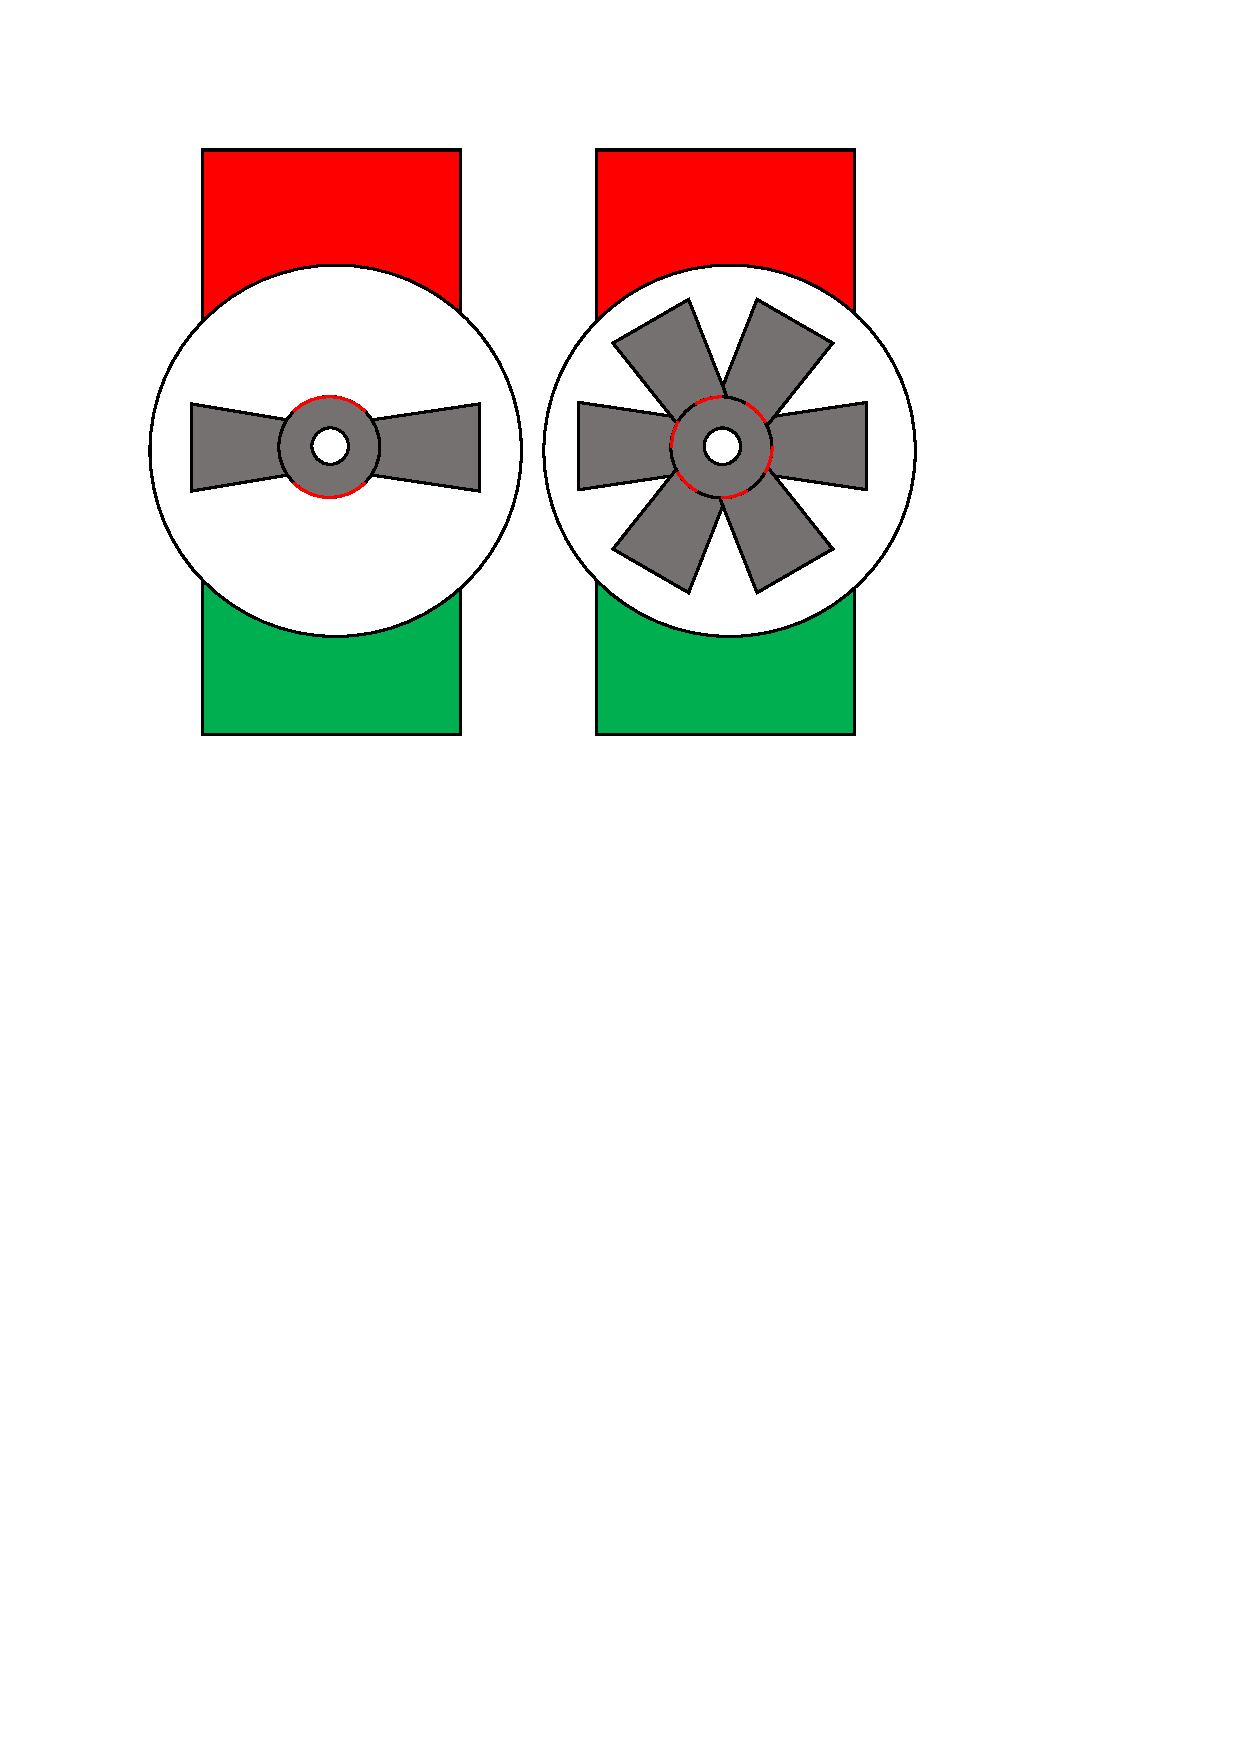
\includegraphics[trim={2cm 15.5cm 0cm 2.548cm}, clip, width=0.8\textwidth]{2polevs6polemotor.pdf}
    \caption[DC motor cross sectional comparison]{This shows a cross sectional comparison between a two pole and six pole motor at various rotation stages. The top left image is labelled showing the: 1. Axle, 2. Commutator, 3. Rotor with windings, 4. Permanent magnets, 5. Stator.}
    \label{fig:2pole_vs_6pole}
\end{figure}

A basic DC motor consists of a stator, a rotor, a commutator, an external magnetic field, brushes, bearings and a shaft. A DC power supply is connected across the brushes, transmitting power through the commutator into windings around the rotor. The current flowing through the windings interacts with the permanent magnetic field producing a Lorentz force, resulting in a torque across the windings,
%reference lorentz
\begin{equation}
    F = I L \times B~,
    \label{Lorentz}
\end{equation}

where $F$ is the turning force, $I$ is the current through the wire and $B$ is the magnetic field strength.

As the rotor spins away from a position with the windings perpendicular to the magnetic field, the torque is reduced. To allow a rotational force over the full revolution, commutators invert the current flow periodically. 

In the simplest possible motor, the rotor is composed of only one set of windings, with a split ring commutator inverting the power supply every half rotation. A more efficient model is to have multiple windings that receive power throughout different stages in the rotation shown in Figure.~\ref{fig:2pole_vs_6pole}. 

At the beginning of the cycle of the two pole motor, the permanent magnetic field is perpendicular to the windings, giving a maximum torque. After one quarter rotation, the windings are parallel to the field. This provides no torque and there is a momentary loss in power as the current is inverted by the commutator. The motor continues to spin due to the momentum gained in the initial stage of rotation until the current is inverted, when torque is regained. For the six pole motor, there is initially a maximum torque supplied by the red marked windings, which decreases to zero at the quarter rotation stage. Unlike the two pole motor, this loss of torque is compensated for, by an increase in torque of the two yellow windings. The torque provided here is more constant than the simple two pole motor, however still not perfectly continuous. An increase in the number of poles increases the continuity of rotation.

The brushes of a motor can be either spring loaded carbon rods, or copper strips pressed against the commutator. Carbon rods are far more efficient and less damaging to the motor, the reasons for this will be discussed further. With advancements in technology, brushless DC motors are becoming increasingly popular, removing the inefficiencies induced by the traditional brushes. 

Mechanical components, such as the bearings, shaft or motor housing are prone to physical damage. This could be due to either physical trauma or a contamination within the motor during operation. Failure of this type would need heavy repairs, with sometimes expensive replacements necessary, it is therefore important to diagnose any unhealthy running motor to minimise the damage.

The contact microphones \footnote{CM-01B Contact Microphone Datasheet: \url{http://docs-europe.electrocomponents.com/webdocs/142c/0900766b8142cdbe.pdf}} used are highly sensitive vibration sensors which record vibrations from 8 Hz to 2.2 kHz. This is done at a sampling rate of 1500 Hz which is a high enough frequency given the motors tested all had fundamental frequencies between 50 and 300 Hz. Three sensors were used for each reading and were placed on the x, y and z axes with x and y parallel to the shaft and z perpendicular. 

\begin{figure}[t]
    \centering
    \begin{circuitikz} 
    \draw (0.9,0.75) node[left] {5 V};
    \draw (5.5,0) node[left] {2};
    \draw (5.5,1) node[left] {1};
    \draw (5.5,-1) node[left] {3};
    \draw (10.5,0) node[left] {V$_2$ out};
    \draw (10.5,1) node[left] {V$_1$ out};
    \draw (10.5,-1) node[left] {V$_3$ out};
    \draw
    (0,0) to[battery]  (1,0)
          to[generic]  (9,0) -- (9,0)
          to[short,-o] (9,0)
    ;
    \draw
    (2,0) to[ground] (2,1)
          to[generic] (8,1) -- (8,1)
              to[short,-o] (9,1)
    ;
    \draw
    (2,0) to[ground] (2,-1)
          to[generic] (8,-1) -- (8,-1)
          to[short,-o] (9,-1)
    ;
    \draw
    (8,1) to[short] node[ground] {} (8,-3)
    ;
    \end{circuitikz}
    \caption[Sensor Circuit Board]{The circuit required to record data. Vibrations recorded by the contact microphones from an analogue output, convert to digital using a National instruments DAQ box.}
    \label{fig:circuit_diagram}
\end{figure}

The vibrational data collected by the contact microphones provided an analogue output, which when passed through a NI multifunction DAQ\footnote{NI USB-6009  Multifunction DAQ USB Device, Datasheet: \url{http://www.ni.com/datasheet/pdf/en/ds-218}}, could be converted and saved as a csv file. The circuit diagram showing the configuration of components is displayed in Figure.~\ref{fig:circuit_diagram}. This was produced using a Veroboard.

The rotation speed of a motor's shaft can provide a lot of information about the running health of a motor. Measurements of rotation speed can be obtained through the use of a rotary encoder \footnote{Three Channel Optical Incremental Encoder, Datasheet: \url{https://www.broadcom.com/products/motion-control-encoders/incremental-encoders-code-wheels/aedb-9140-a14}} which is fitted to the rotating shaft. The encoder is a composed of a codewheel and an emitter/detector module. As the disk spins, the apertures periodically block or allow the light to pass from the emitter to detector, converting the rotary shaft motion into a digital output. The rotary disk has three sections for varying level of accuracy, one channel outputs once per revolution, the others providing higher resolution with 500 counts per revolution.

The quadrature output of the rotary encoder allows monitoring of the shaft rotation speed with time, allowing investigation into certain failure modes such as slipping. This piece of equipment is relatively invasive compared to the contact microphones, as it requires fixing to the shaft, limiting space for operational output. 

\subsection{Calibration Tests}

In order to determine which frequency components were from the motors and what was simply noise (unwanted signal), calibration tests were run for each motor. This involved recording data whilst the motor was off. 

\begin{figure}[t]
    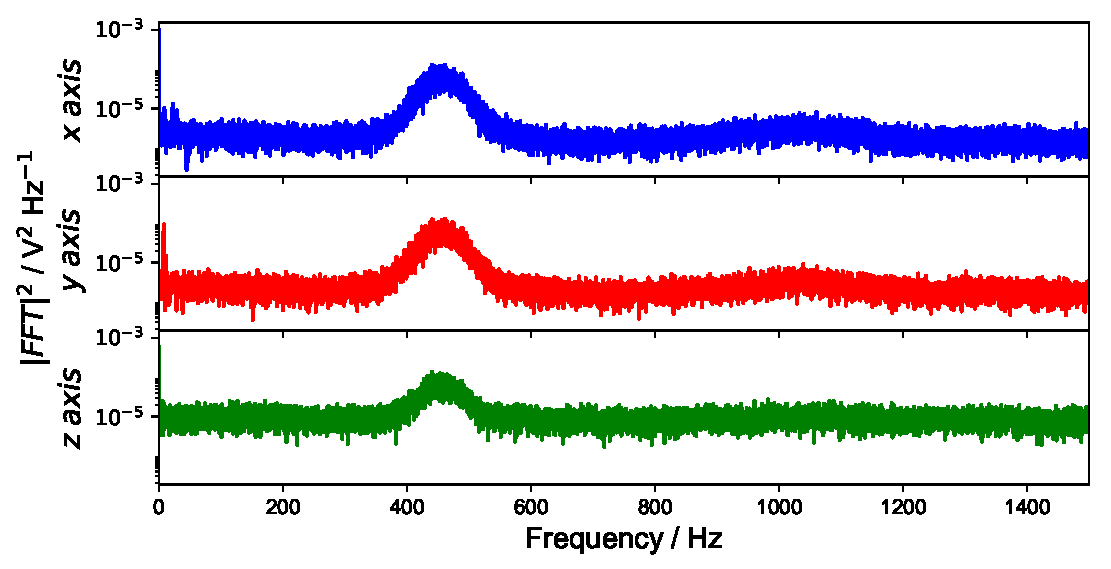
\includegraphics[width=1.0\textwidth]{fig/freq_large_0V.pdf}
    \caption[Calibration Frequency 1]{The Fourier spectra in the x, y, and z axes for Motor A at 0 V.}
    \label{fig:freq_large0V}
\end{figure}

Figure.~\ref{fig:freq_large0V} shows the frequency spectra for a calibration test with Motor A. 

This peak was originally attributed to ambient sounds in the lab, however repeat measurements were conducted with the microphones not powered and the peaks still persisted. This indicates that the source of the noise is from the DAQ box or electronics. 

The position of this peak appeared to vary randomly between approximately 300 and 1000 Hz, for different data sets. The reason for this is unknown, however for most cases the peak was at a higher frequency compared to the fundamental frequencies of the motors, and was often orders of magnitude smaller. 

\subsection{Baseline Tests}

\begin{figure}[t]
    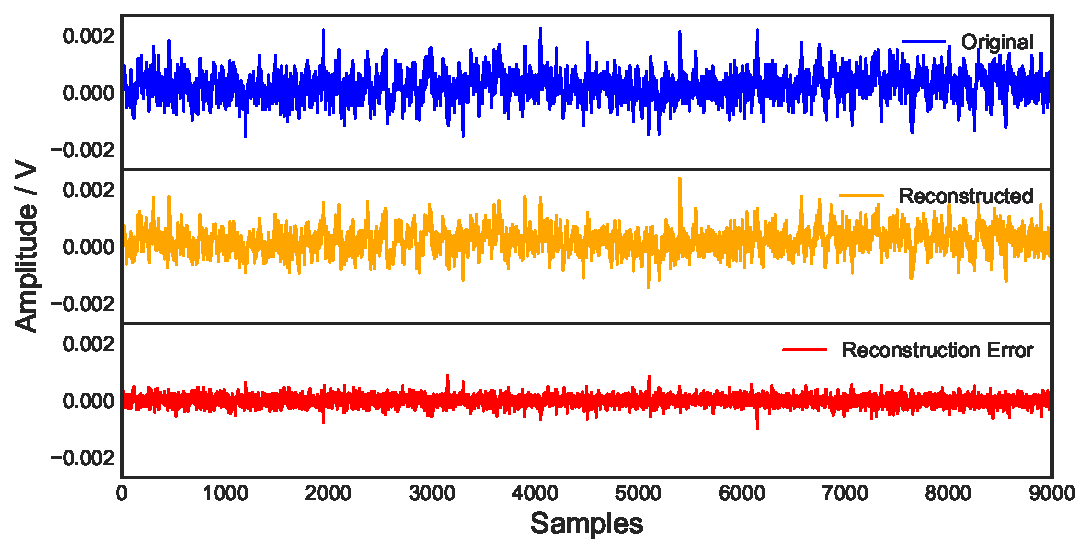
\includegraphics[width=1.0\textwidth]{fig/kmeans_large_4Vnowater.pdf}
    \caption[K-means Large Motor Reconstruction No Water]{K-means reconstruction applied to three seconds of data from Motor A running at 4 V. Top: the original testing data. Middle: the reconstruction using K-means. Bottom: the reconstruction error between the reconstructed and original signal.}
    \label{fig:kmeans_large4V}
\end{figure}

\begin{table}[]
    \centering
    \begin{tabular}{|p{1cm}|p{1cm}|p{10cm}|}
    \hline
    \textbf{Motor}          & \textbf{Motor Type}        & \textbf{Description}                                                                          \\ \hline
    \multicolumn{1}{|l|}{A} & \multicolumn{1}{l|}{Ungeared} & 12 V motor used to test effects of load/overvoltage.                            \\
    \multicolumn{1}{|l|}{B} & \multicolumn{1}{l|}{Geared} & 12 V motor with gear ratio 5/288. Used to test degradation of gears through rust/dirt. \\
    \multicolumn{1}{|l|}{C} & \multicolumn{1}{l|}{Ungeared} & 5-15 V toy motor. Shaft bent to test rotor imbalance.                                \\
    \multicolumn{1}{|l|}{D} & \multicolumn{1}{l|}{Ungeared}   & Motor heated to test overheating effect on coils.                          \\ \hline
    \end{tabular}
    \caption[Motor Descriptions]{All four different motors that were used in experiments, alongside a short description of their properties.}
    \label{motor_table}
\end{table}

Figure.~\ref{fig:kmeans_large4V} shows the K-means reconstruction of a three second signal using training and testing data both sourced from a `baseline test run'. A baseline test run is data collected from a motor running under its optimum working conditions, with a supply voltage of 12 V for all motors apart from Motor C (see Table.\ref{motor_table}). The motor would be free from an applied load, any damage, or anything else that could cause the manifestation of an investigated failure mode. A baseline test run provided us with the `normal' data that one could train various models with, on the assumption that the nature of the vibration data is wholly representative of the motor's intended behaviour.

The first three seconds of the baseline test run was used as training data and the second three seconds used as fitting data. This was done to check if the synthetic segments could be used to recreate a later section of the same baseline run with minimal reconstruction error. 

\subsection{Overheating}

\subsubsection{Description of Failure Mode}

Overheating is widely regarded as the most common cause of motor failures, with many other types of motor deterioration leading to overheating. This is such a substantial problem that a rise of just 10 $^o$C above the regular running temperature causes the life expectancy of the motor to halve. The life span is halved once again for every 10 $^o$C the temperature is raised further.%ref?

The problem arises as, during overheating, the varnish covering the metal wires begins to melt \cite{wagner1993effects}. If this occurs at two points of wires that are in contact, the coil of the motor can short circuit.

%(Gears Removed motor)

In order to induce motor failure, motor D, shown in Figure.~\ref{fig:hotplate_motor}, consisting of 7 coils separately providing power was placed on a hotplate, heated to 150 $^o$C, for one hour. This was compared to the assumed usual running temperature of 60 $^o$C, meaning that just one hour on the hot plate equated to 512 hours of regular use.

For this failure mode, only one coil was in direct contact with the plate so as only to damage that coil, leaving the others, ideally, with little impairment. Despite the fact that some heat would obviously be conducted through the motor, the effect of this was considered to be minimal with respect to the effect on the targeted coil.

The result of just one coil being broken is that there would be a brief loss of power in the motor when this coil was in contact with the brushes. Therefore the speed of revolution would no longer be uniform. This can cause other problems to occur in the motor such as damage to the bearings. 

In addition to this, the motor was placed in an oven at 200 $^o$C for two hours to cause extensive damage to all the coils evenly. This equates to over 30,000 hours of running in regular conditions. This was considered sufficient to bring the motor very close to failure given the typical life span of a 12 V motor is just 5000 hours \cite{jones1973selecting}.
Data was then collected for one minute to find any lasting damage.

In case this did not result in the targeted coil breaking entirely, a further experiment was devised that simulated this effect. To inhibit just one coil, one of the coils was cut. It was then observed that the rotation speed was not constant with no power being given to the motor for $({2}/{7})$th of the time - due to the fact that neither of the two brushes could be in contact with the broken coil. Further coils were cut and the speed was noted to become even more erratic. Once four had been broken, the motor was unable to run at all as there was never a point where two brushes were in contact with working coils.

\begin{figure}[t]
    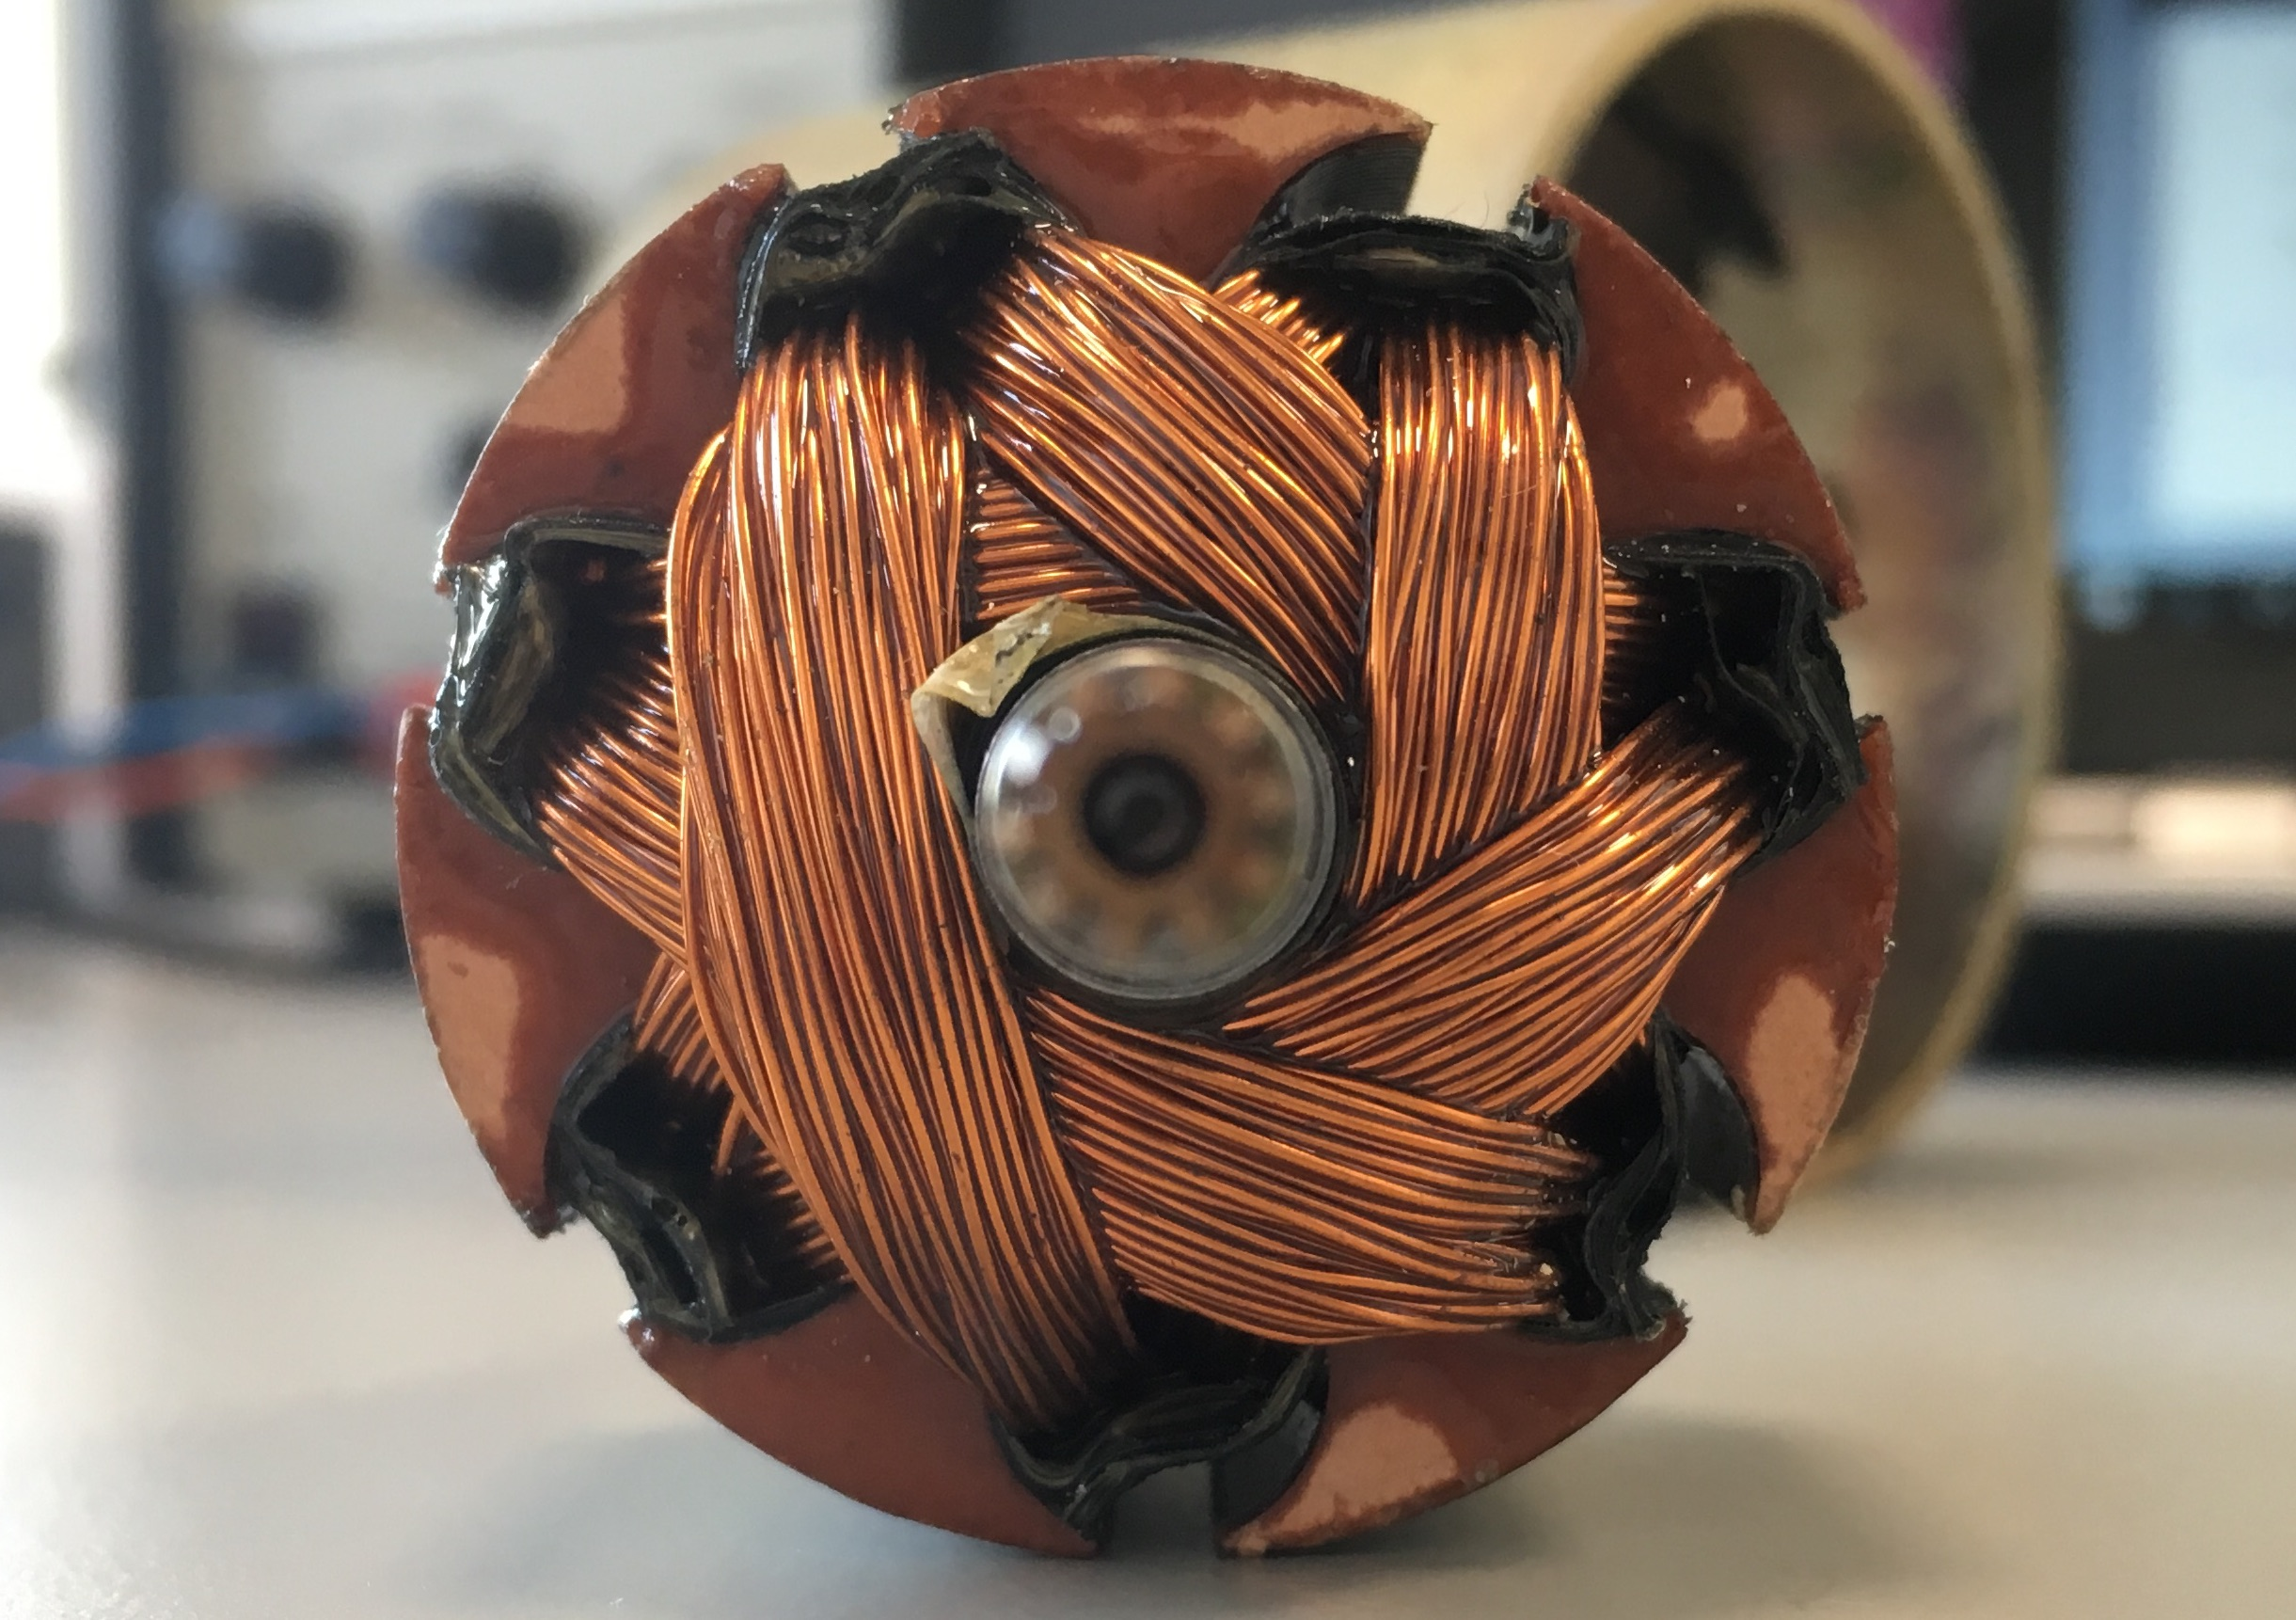
\includegraphics[width=1.0\textwidth]{fig/Gears_Removed_Inside.JPG}
    \caption[Inside Workings of Motor D]{The inside of the Gears removed motor showing the 7 separate coils, one of which was placed directly on the hotplate at 150 $^o$C for one hour to induce failure.}
    \label{fig:hotplate_motor}
\end{figure}

%Need references from papers for this

\subsubsection{Application of Anomaly Detection}

\begin{figure*}[t!]
    \centering
    \begin{subfigure}[t]{0.5\textwidth}
        \centering
        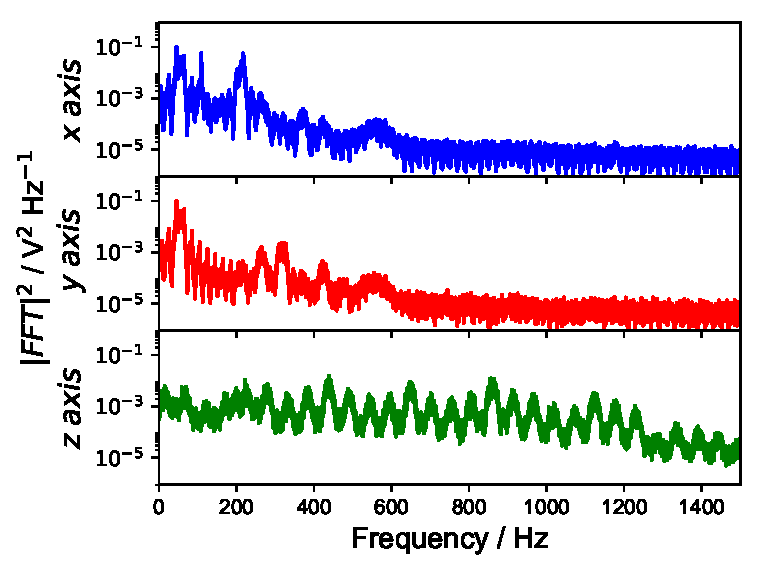
\includegraphics[height=2.5in]{freq_gears_removed_baseline.pdf}
    \end{subfigure}%
    ~ 
    \begin{subfigure}[t]{0.5\textwidth}
        \centering
        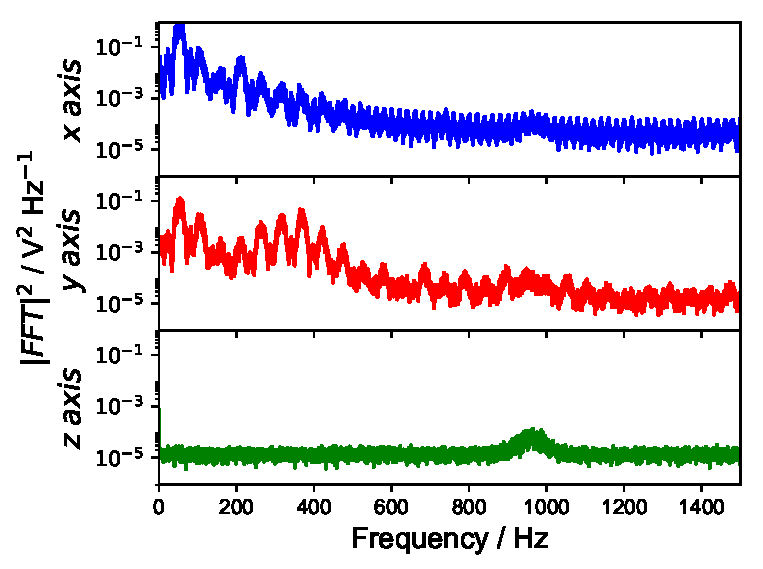
\includegraphics[trim = {2.61cm 0 0 0}, clip,height=2.5in]{freq_gears_removed_oven.pdf}
    \end{subfigure}
    \caption[Fourier Plot Overheating]{Fourier spectra for the gears removed motor in all three axes. Left: baseline test at 12 V. Right: motor run at 12 V after being placed in oven at 200 $^{\circ}$C for 2 hours.}
    \label{fig:overheating_fourier}
\end{figure*}

Time domain anomaly detection methods were applied to the data recorded after the motor had been placed on the hotplate, however none of the time domain tests gave an indication of anomalous behaviour. The time domain tests did not indicate any anomalies after the motor had been placed in the over, either. 

The Fourier spectra did indicate clear signs of abnormal motor behaviour after overheating. 

Figure.~\ref{fig:overheating_fourier} shows the Fourier spectra of Motor D for baseline data and data recorded after overheating from the oven. Visual inspection of the spectra shows very distinct differences between the two sets of spectra. 

There appears to be a greater dynamic range between peaks for the Fourier spectra of the overhead motor, particularly in the y axis. The y axis also appears to have a broad peak between $\sim200$ - $400$ Hz, which could be as a result of the varying rotation speed present after the motor was overheated, creating a wider peak as the frequency changes over time.

Another observation is that the average power spectral density is much higher in the x and y axes after overheating. This is expected as when the motor is not operating at ideal conditions, more power is transferred to the vibrations and sound of the motor.

The z axis shows the same spectra to that of the calibration test. This suggests that there was a fault in this particular sensor recording for this set of data.

\begin{table}[t]
\centering
\begin{tabular}{|c|p{1.2cm}p{1.2cm}p{1.2cm}|p{1.2cm}p{1.2cm}p{1.2cm}|p{1.2cm}p{1.2cm}p{1.2cm}|}
\hline
  & \multicolumn{3}{c|}{\textbf{Baseline}}                    & \multicolumn{3}{c|}{\textbf{Hotplate}}                & \multicolumn{3}{c|}{\textbf{Winding Snipped}}         \\ \cline{2-10} 
  & $A$            & $\mu$           & $\sigma$      & $A$           & $\mu$        & $\sigma$      & $A$               & $\mu$        & $\mu$      \\ \hline
x & $27.2 \newline \pm 0.8$ & $61 \newline \pm 6$      & $8.1 \newline \pm 0.5$ & $7.7 \newline \pm 0.3$ & $966 \newline \pm 9$  & $6.9 \newline \pm 0.3$ & $4 \newline \pm 3$         & $680 \newline \pm 20$ & $11 \newline \pm 1$ \\
y & $27.6 \newline \pm 0.8$ & $52.3 \newline \pm 0.5 $ & $8.5 \newline \pm 0.5$ & $49 \newline \pm 4$    & $320 \newline \pm 4$  & $6.2 \newline \pm 0.2$ & $4 \newline \pm 3$         & $680 \newline \pm 20$ & $10 \newline \pm 1$ \\
z & $8.3 \newline \pm 0.3$  & $673 \newline \pm 33$    & $6.6 \newline \pm 0.2$ & $13 \newline \pm 13$   & $1172 \newline \pm 5$ & $100 \newline \pm 90$  & $0.069 \newline \pm 0.007$ & $703 \newline \pm 5$  & $12 \newline \pm 2$ \\ \hline
\end{tabular}
\caption[Gaussian Fit Parameters for Overheating]{Gaussian fit parameters for the most prominent peak in the Fourier spectrum, in the x, y and z axes of the motor. Parameters are returned for a baseline run, after one of the coils was placed on a hotplate, and when one of the coils was completely snipped. The units of $A$ are $10^{-3}$V$^2$ H$^{-1}$ and the units of $\mu$ and $\sigma$ are Hz.}
\label{table:overheating_table}
\end{table}

Table.~\ref{table:overheating_table} shows the parameters returned when minimising a Gaussian fit to the most prominent peak in each axis of motor D. A Gaussian was initially fitted to a baseline test run, in which the motor was operated at 12 V under no load, assumed to be its optimum conditions. The data obtained after motor D had been placed on the hotplate is shown in the second column. The third column shows the fitting parameters after one of the motor's windings had been snipped. 

The parameters returned from Gaussian fitting all significantly change after the motor winding was placed on the hotplate, as can be seen in Table.~\ref{table:overheating_table} in the Baseline and Hotplate columns.

The parameters returned from when the overheated motor then had one of its windings snipped changed even further. The fact that the parameters changed between the overheated motor and snipping the windings suggests that overheating the motor did not have a completely debilitating effect on that particular effected winding.

As the Gaussian parameters for the baseline run are not in agreement within their errors with those for the overheated motor, this shows the effectiveness of Gaussian fitting method in detecting anomalous motor behaviour. 

\subsection{Overvoltage and Undervoltage}

\subsubsection{Description of Failure Mode}
An increase in voltage will also cause an increase in current, resulting in more eddy currents in the wires and subsequently heating the motor. As stated earlier, this is a major reason for motor failures. 

Moreover, overvoltaging causes the torque of the motor to increase. The subsequent increased rotation speed leads to the rotor slipping. In order to reduce this slip, the motor will then draw an even greater current further contributing to the overheating effect. As well as this, a greater rotation speed will increase friction and will wear down bearings and brushes. Just a small increase in voltage can result in a large amount of damage as,

\begin{equation}
\tau \propto V^2,
\label{Torque}
\end{equation}

where $\tau$ is torque and $V$ is voltage.

In addition to the detrimental effect of overvoltaging, undervoltaging can be just as destructive. In fact, the effect of slipping is even more prominent when a motor is not given enough power and leads to more overheating.

%12V motor

The effect of overvoltaging  was investigated by running motor B at increasingly high voltages ranging from 12 V to 30 V. This was done for just one minute each time and was used to find the immediate effects of overvoltaging a motor.
    
%Large Motor

A second motor, motor A, was run at 30 V for one hour. In this instance, the temperature of the bearings reached 90 $^o$C; this demonstrates the extreme effects of overvoltaging a motor. Readings could not be taken during this run as the sensors are only able to operate %Need synonym
up to 60 $^o$C. %Correct???
Therefore, readings were taken before and after the one hour run. This allowed us to explore the long term effects of overvoltaging a motor.

%Undervoltage experiment (large motor)

In order to investigate the effects of undervoltaging a motor, data was collected when running motor A from 1 V through to 5 V, in 1 V instalments. The speed of rotation could be seen to be irregular, providing evidence that the rotor was slipping. This speed was taken using the rotary encoder, as mentioned earlier. %data?

%Again need references.

\subsubsection{Application of Anomaly Detection}

%COMMENTED OUT TO ONLY TALK ABOUT ONE FIGURE
%\begin{figure}[t]
%    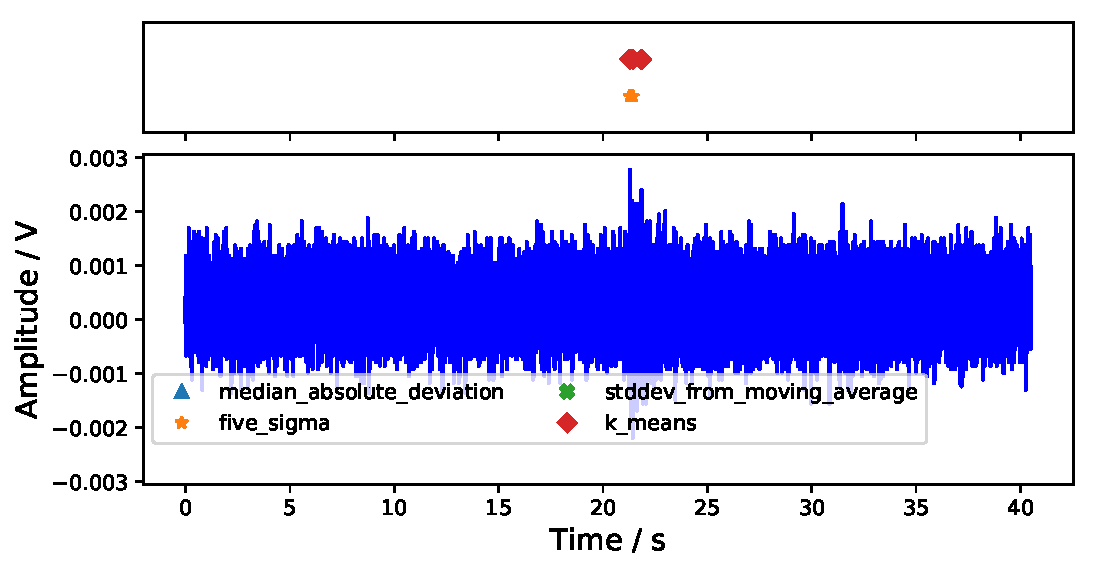
\includegraphics[width=1.0\textwidth]{fig/large_2V_nowater_large_12V.pdf}
%    \caption[Undervoltage of Large Motor1]{Waveform for the large motor running at 2V, significantly below optimum voltage.}
%    \label{fig:largemotor_2V}
%\end{figure}

\begin{figure}[t]
    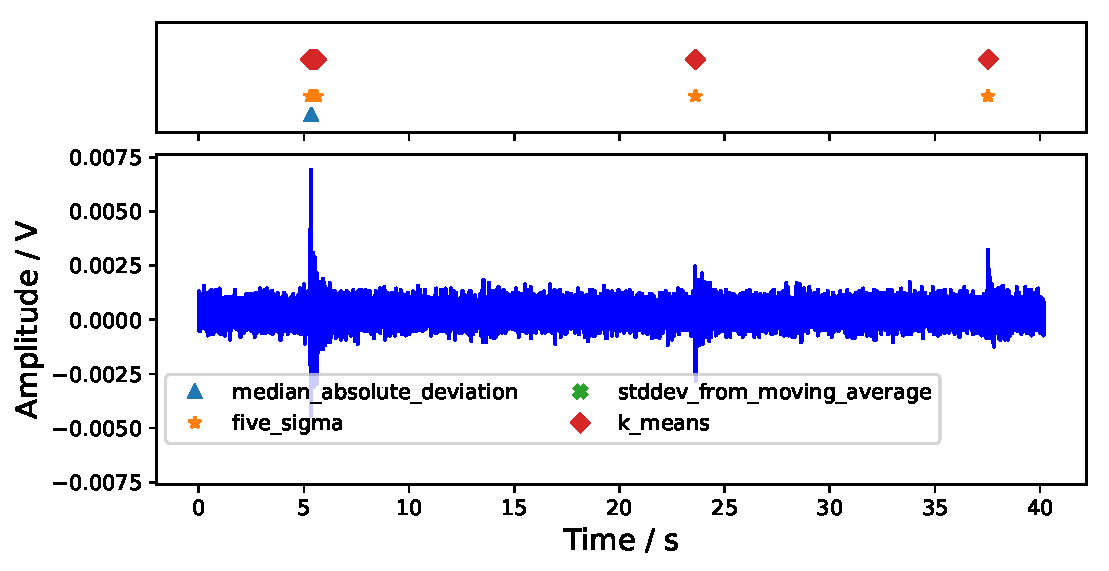
\includegraphics[width=1.0\textwidth]{fig/large_1V_nowater_large_12V.pdf}
    \caption[Undervoltage of Large Motor]{Waveform for Motor A running at 1 V, significantly below optimum voltage. Anomaly detection trained against 12 V baseline data, assumed to be the motor's optimum working conditions.}
    \label{fig:largemotor_1V}
\end{figure}

%refer in the text that when this test is tested against baseline data, it doesn't return any anomalies therefore this undervoltage is the thing causing the anomalies. all anomaly method detected the anomalies. EXCEPT from stdev_from_mov_av. WHY? which anomaly detection caught is sooner? zoom in it could potentially be something to ask jake and rob more, what could be the physical reason of these spikes when it's being unvoltaged.
When the anomaly detection methods were tested against the baseline data for Motor A, no method detected any anomalous data points within the set. Therefore one can assume that on the test data presented in Figure.~\ref{fig:largemotor_1V}, only the effects of the motor running below the optimum voltage were flagged up by the detection methods. 

It is also important to note that all anomaly detection methods correctly identified the anomalies but Standard Deviation from Moving Average, which failed to detect any of the anomalies caused by the under-voltage of the motor. This could be due to the chosen value of $4\sigma$ within the detection code being too high for the data set, thereby filtering out potential results.

Each index within the data on which anomalous results are flagged up seem to be similar across each method, indicating no speed advantage between them, however, Median Absolute Deviation seems to stop flagging the anomaly before K-means and Five Sigma. %why?

\begin{figure}[t]
    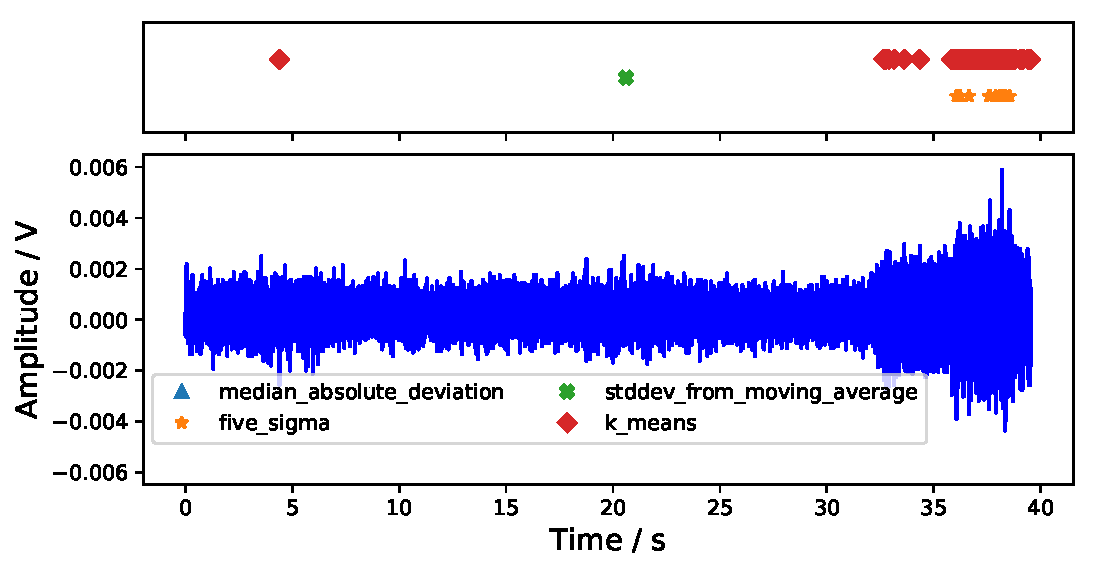
\includegraphics[width=1.0\textwidth]{fig/large_30V_large_12V.pdf}
    \caption[Overvoltage of Large Motor]{Waveform in the x axis for Motor A running at 30 V, significantly above optimum voltage. K-means was trained against 12 V baseline data, assumed to be the motor's optimum working condition.}
    \label{fig:largemotor_30V}
\end{figure}

%NEED TO TALK ABOUT OVERVOLTAGE HERE
%Apparently motor voltage fluctuated as motor got hot. This very nicely shows how amplitude gradually increases towards end, and is found by the majority of time domain anomaly detection methods. 
Figure.~\ref{fig:largemotor_30V} displays the effects of running the motor far above the optimum voltage of 12V. The voltage fluctuated toward the end of the testing data due to overheating of the motor, but was originally set at 30 V. It clearly shows anomalous data corresponding with the heating of the motor as a direct result of over-voltage. Most time domain anomaly detection methods flagged these results with K-means test detecting both before and after the Five Sigma test. This shows a clear advantage of using the K-means test as if the motor was switched off immediately as the first few anomalies were detected by the K-means test, the motor would not continue to operate at such high temperatures and fluctuating voltages which would potentially damage the motor.

\subsection{Load}

\subsubsection{Description of Failure Mode}
The presence of a load puts a large amount of stress on the motor. As the motor struggles to reach the desired voltage, a greater current is drawn, which leads to overheating.
        
There are many ways of adding a load to a motor, but attaching a fan immersed in water was chosen due to the ability to vary the load through using fans of different widths (1 cm, 2 cm and 3 cm).
    
Initially the test was done on motor B. A gear ratio of ${5}/{288}$ was found by counting the teeth of each cog and finding the speed of the connecting cog. This meant that the speed of the shaft, $\omega_1$, is much slower than the speed of the axle, $\omega _2$,

\begin{equation}
\omega_1 = \frac{5}{288} \omega_2.
\label{eq:gear_ratio}
\end{equation}

This increased the torque of the shaft and resulted in the motor being able to deal with a greater load. It was even able to run at 30 V for the thickest fan.

A test was then conducted for motor A. This time the motor could only reach a maximum of 4 V when the 1 cm fan was in use. This is evidence that as a load is added, a greater current is required to achieve a power that is large enough. A 10 A power supply was used for this experiment and this was the limiting factor, preventing the voltage from increasing further.

\subsubsection{Application of Anomaly Detection}

\begin{figure}[t]
    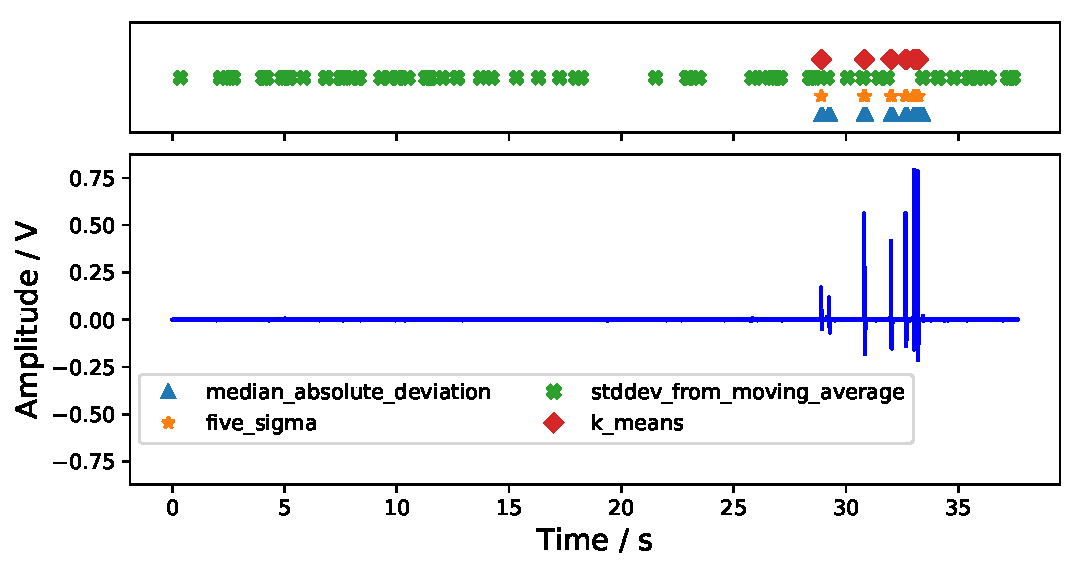
\includegraphics[width=1.0\textwidth]{fig/large_4V-9A_water_large_12V.pdf}
    \caption[Anomaly Plot Large Motor under Load]{Waveform for Motor A running under applied load from water bucket at 4 V. Anomaly detection trained against 12 V baseline data, assumed to be the motor's optimum working conditions.}
    \label{fig:largemotor_water4V}
\end{figure}

Figure.~\ref{fig:largemotor_water4V} shows the anomaly tests being applied to data recorded when Motor A was running under an applied load.

The standard deviation from moving average test looks at more short term changes along the time series. The algorithm involved calculates the mean and standard deviation of a `chunk' of data, and evaluates novelties in the data on a more local level. Larger spikes at the 30 second mark in Figure.~\ref{fig:largemotor_water4V} has meant that the fluctuations the test identified as anomalies are not visible.

The spikes of data displayed in Figure.~\ref{fig:largemotor_water4V} seem to be due to the sub-optimum voltage that the motor is running at as a result of the water resistance applied to the fans, and are indicative of catastrophic anomalies that significantly change the performance of the motor. These anomalies may be due to the rotor slipping due to the applied load, or due to water turbulence. Regardless, all applied anomaly detection methods detected these with ease.

All other anomaly detection methods, barring standard deviation from moving average, provided meaningful pointers as to where the anomalous data is recorded. This is due to them very clearly only flagging the visible spikes.


%std_dev_mov_av goes crazy. this looks for local changes rather wheras other threshold test slook at the data as a whole, this is why other stat tests only look at the spikes and this methods finds stuff for low amplitude data.
%spikes are detected all by the anomaly tests. which one does it better? Link in physically to what the spikes actually mean...

\subsection{Rotor Imbalance}
As the rotor spins within the motor, it is important for the weight to be evenly distributed around the central axle. Any imbalance present can cause the rotor to shift in position toward the areas of concentrated mass \cite{xu1994vibration}. As a motor runs, increased levels of vibrations are produced with the frequency of the vibrations matching the shaft rotation speed. This unnecessarily increases the stress on the bearings and, in extreme cases, this can cause contact between the rotor and the stator. This increased strain on the bearings causes a larger friction, not only reducing the efficiency of the motor but also damaging the bearings. This can lead to complicated maintenance operations that would be otherwise unnecessary for a properly aligned motor.

If there is contact between the rotor and stator, there is again an increase in friction. This is often a larger frictional force, decreasing the efficiency further, but also generating large amounts of heat. When operated in this condition for long periods of time, this can cause overheating, as discussed above. As the rotor spins against the stator, the friction is capable of causing unwanted damage to both the rotor and the stator. In the case that this force is large enough, the permanent magnets could become detached from the stator, ultimately resulting in a failed motor.

Some possible causes of an imbalanced motor include: uneven wear through use, design or assembly errors, and an eccentricity of the rotor or any physical damage distorting components. Observing additional, unexpected frequencies could be due to an imbalance within the motor, and as such are a warning sign to the decline in health of the motor. 

%\begin{figure}
%    \centering
%    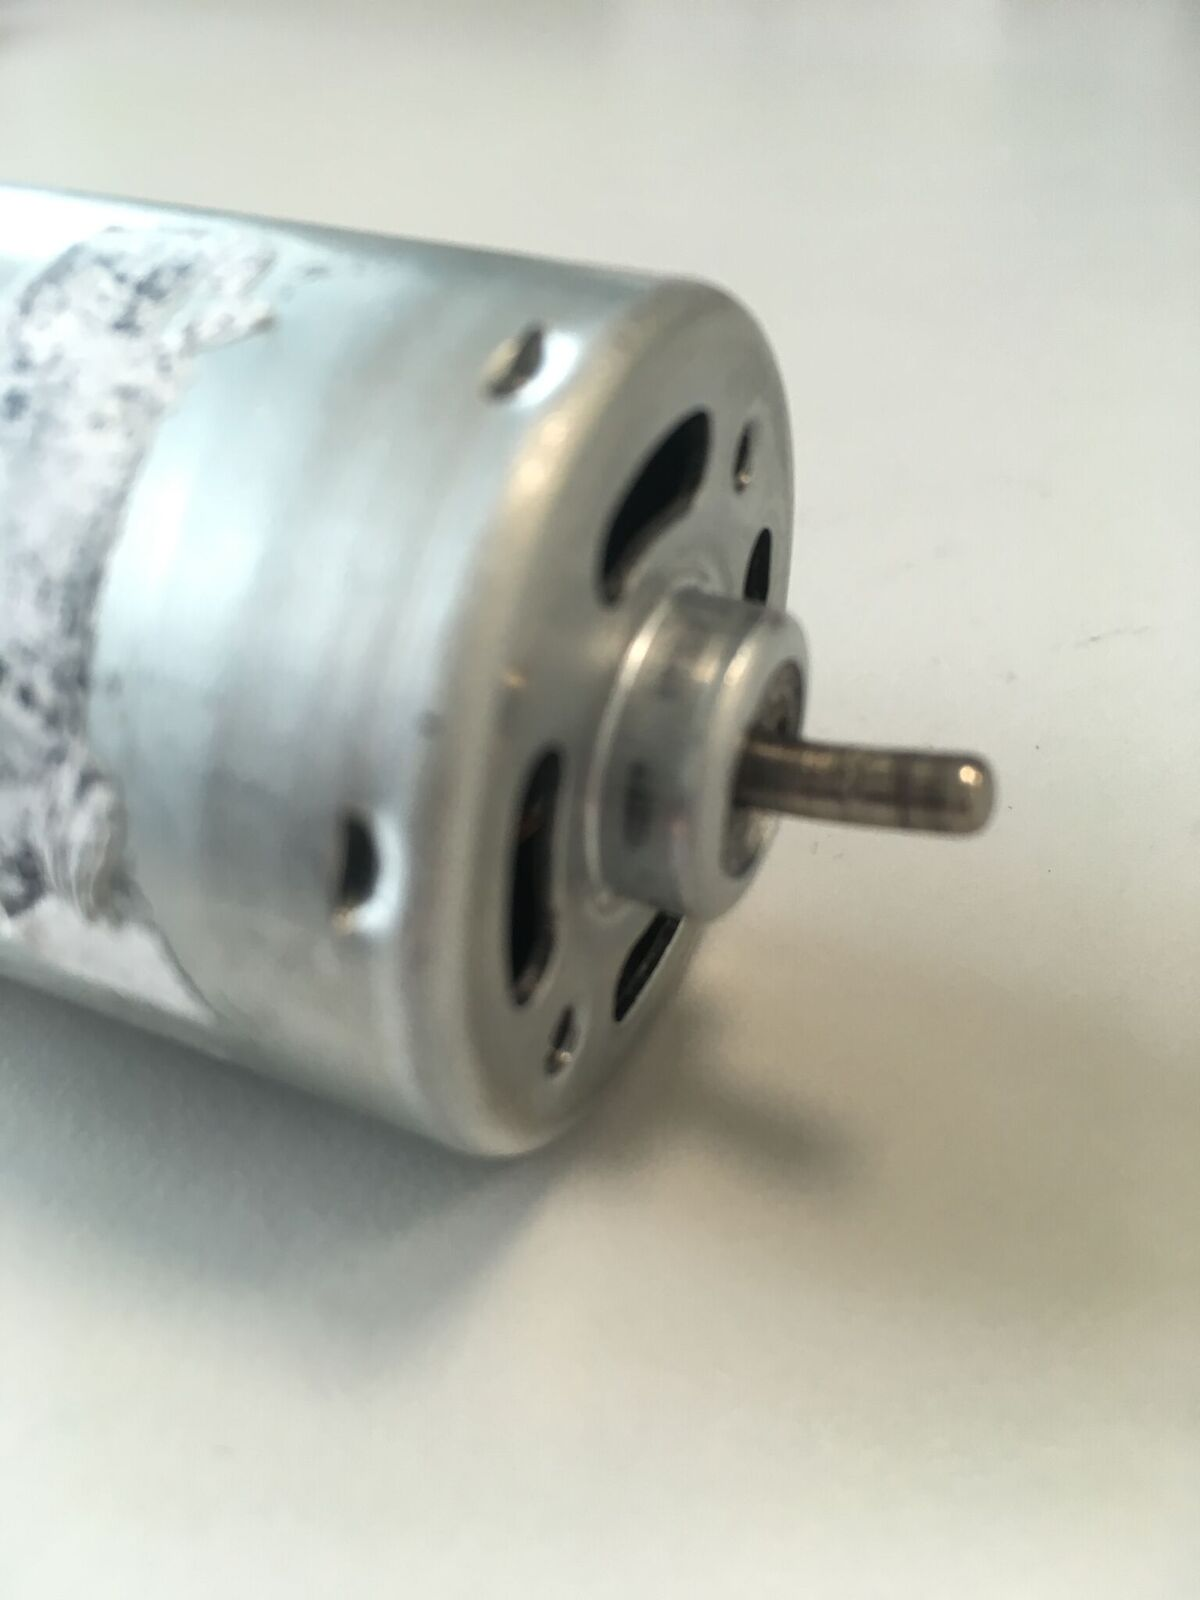
\includegraphics[trim={0cm, 15cm, 0cm, 8cm}, clip, width=0.5\textwidth]{bentshaft1.jpg}
%    \caption[Misaligned Motor Shaft]{Small motor with misaligned shaft}
%    \label{fig:bentshaft}
%\end{figure}

To simulate an imbalanced motor, the shaft of motor C was bent with varying severities. 
%(See Figure.~\ref{fig:bentshaft}.)
%Removed for space and aesthetics
As with all motors, it is impossible to attain a state of perfect balance, so small bends are expected in any initial baseline test. As the angle of the shaft from the normal was increased, the motors health deteriorated greatly. At large bends, the frictional force became so large that the motor required an initial force to start movement. This could represent a heavy contact between the rotor and the stator. 

\begin{figure*}[t!]
    \centering
    \begin{subfigure}[t]{0.5\textwidth}
        \centering
        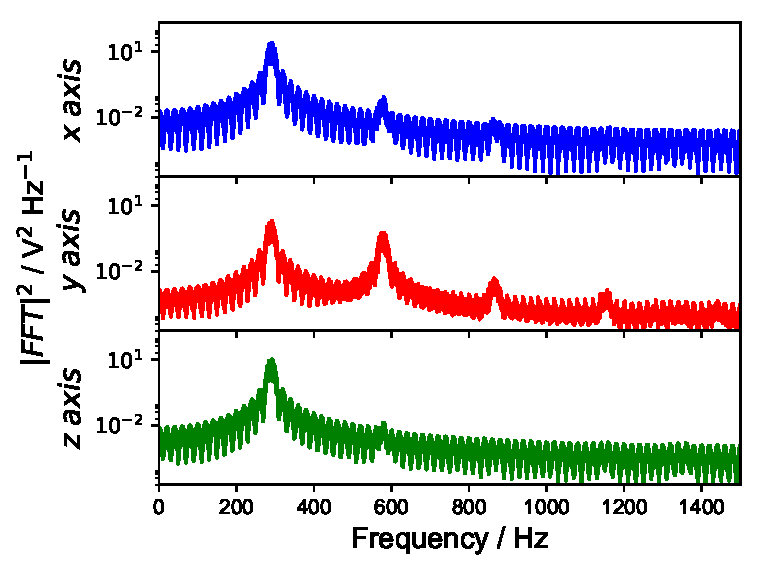
\includegraphics[height=2.5in]{small_baseline.pdf}
    \end{subfigure}%
    ~ 
    \begin{subfigure}[t]{0.5\textwidth}
        \centering
        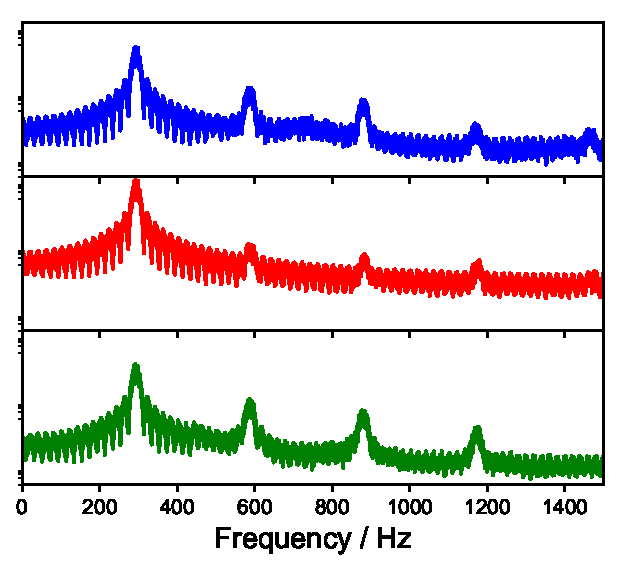
\includegraphics[height=2.5in]{small_misaligned_3.pdf}
    \end{subfigure}
    \caption[Fourier Plot Misaligned Shaft]{Fourier spectra for the small motor in all three axes. Left: baseline test at 15 V. Right: motor run at 15 V with bent shaft.}
    \label{fig:bent_shaft_fourier}
\end{figure*}

%Talk about very distinct harmonics appearing with bent shaft. Physically why would this be?
Figure.~\ref{fig:bent_shaft_fourier} displays the Fourier spectra of Motor C for baseline data and data recorded once the shaft was bent to its largest extent. As clearly visible in the figure, the $x$ and $z$ axis displays very distinct harmonics after the shaft is bent. This is most likely caused by knocking and unwanted contact within the motor, reducing the effectiveness of the motor's operation.

%Time domain tests find continuous anomalies with the K-means and the five sigma test, but these tests also find anomalies in the baseline test, indication possible false positives. For rotor imbalance, frequency analysis definitely seems more effective. 

\subsection{Brush Damage}

\subsubsection{Description of Failure Mode}
The brushes of a DC motor are a vital component, key to the proper working of the motor, allowing a DC power supply to provide an almost constant driving force throughout the entire revolution of the motor. The stationary brushes, combined with the rotating commutator attached to the rotor, periodically inverts the power supply throughout the revolutions. The commutator is composed of strips of conducting metal, usually copper, placed around the rotor. The strips of copper supply the current from the spring loaded brushes to the windings.  Without this periodic inversion of current direction through the windings, the motor would fail to spin and, as such, a good contact between the face of the brush and the commutator is necessary. 

The main cause of damage to the brushes of a DC motor usually occurs during maintenance. The soft surfaces of the carbon brushes can be easily scratched if not handled correctly \cite{hamilton2000dc}. It is also possible that dirt can enter the motor housing during operation, which if found between the brush and the commutator, can cause heavy damage. In order to induce this type of failure mode, the brushes of motor A were treated with a heavy grit sandpaper, leaving the surface very rough, see Figure.~\ref{fig:brush_damage}.

\begin{figure}[t]
    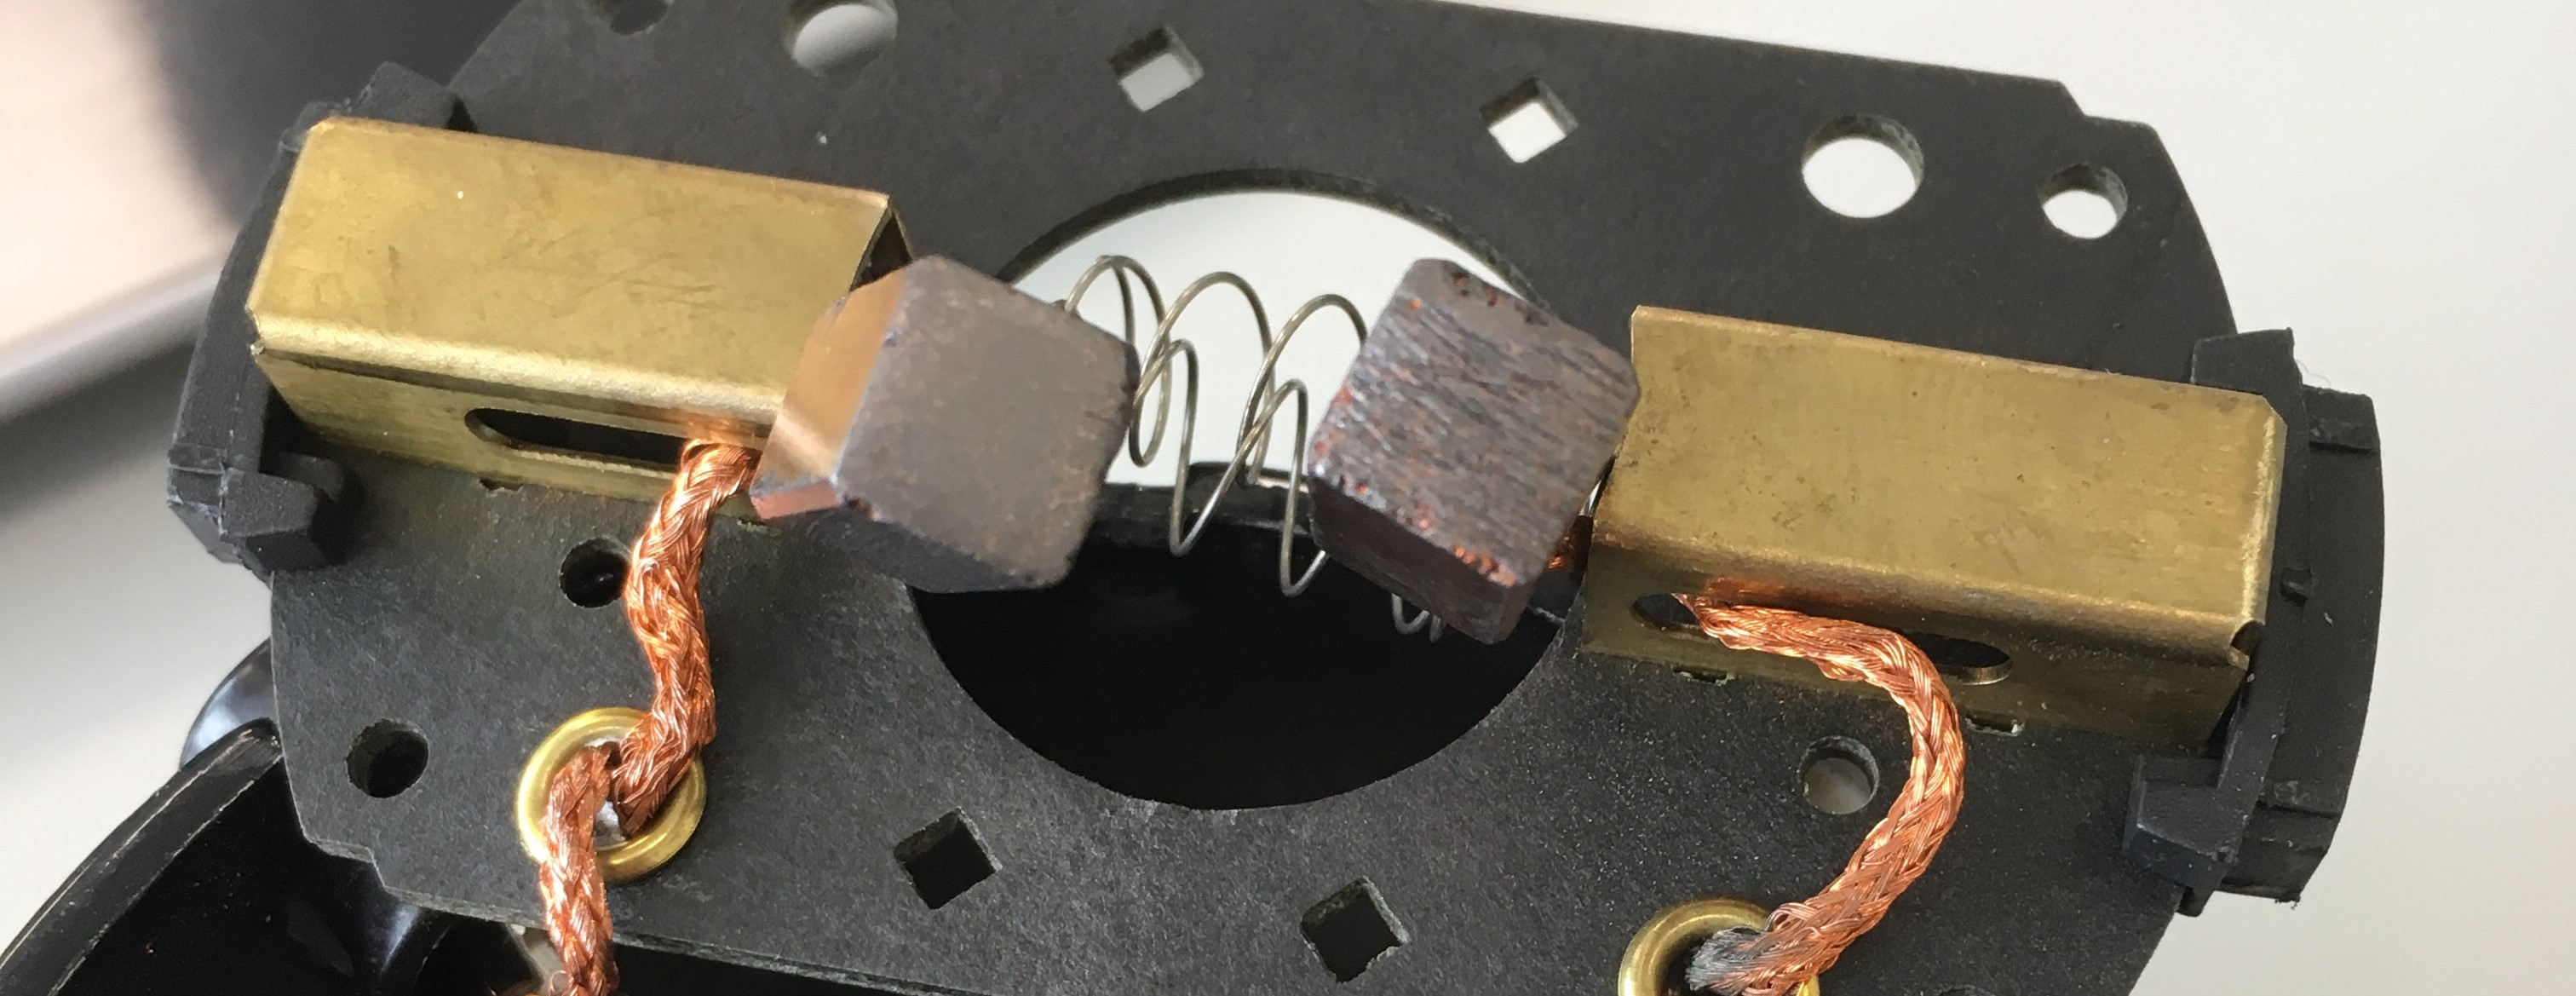
\includegraphics[width=1.0\textwidth]{fig/brush_comparison.jpg}
    \caption[Brush Damage]{Comparing the left and right brushes before and after deliberate manual damage.}
    \label{fig:brush_damage}
\end{figure}

It is possible for any imperfections in the surface of the carbon brushes to be removed without intervention during normal operation. As the rotor spins, making contact with the face of the brushes, the friction generated is often capable of reducing the magnitude of the scratches. To investigate this, after the brushes had been damaged, the motor was operated for 30 minutes at 12 V to allow for the possibility of self repair. %FROM ANALYSIS DID THIS WORK? ---- It did indeed --wow thats awesome

The friction within the brushes can cause another failure mode, loss of contact due to reduction in size of the brushes over time. This requires the brushes to be entirely replaced, making brushed motors unsuitable for use in remote locations.

The rough contact between the brush and commutator when damaged can cause sparking, leading to damaged commutators. Replacing the brush on a motor is a relatively simple maintenance task, however replacing the copper strips of a commutator can be more complicated. It is therefore important to ensure that a motor running with damaged brushes is identified immediately, to prevent running in sub-optimal conditions, potentially causing further damage

Due to the flaws in the brushed DC motor model, their use has been declining with the introduction of brushless DC motors. These use an integrated switching power supply, to convert the DC to AC for the motor to run \cite{hanselman2003brushless}. Another alternative is to simply use an AC motor. 
%hammer brush explanaion with picture if data shows it had any meaningful effect?

\subsubsection{Application of Anomaly Detection}

\begin{figure}[t]
    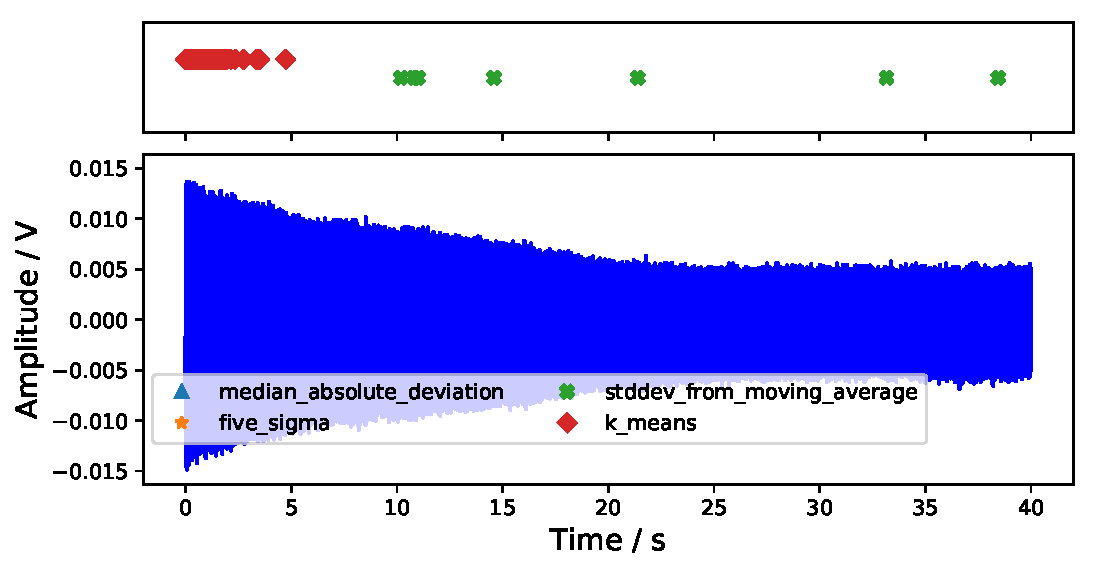
\includegraphics[width=1.0\textwidth]{fig/large_manual_repair_large_12V.pdf}
    \caption[Anomaly Test Brush Damage]{The waveform in the x axis for Motor A after brush damage, showing the process of self-repair.}
    \label{fig:largemotor_brushdamage}
\end{figure}

Figure.~\ref{fig:largemotor_brushdamage} highlighted the motor vibrations becoming less and less of an anomalous nature during the process of self repair. This is observed by the frequency of K-means anomaly alerts steadily decreasing as the motor returns to a state that is more in agreement with the baseline data it has been trained against. This is evidence that the K-means test can successfully distinguish anomalous and normal regimes over the course of a continuous measurement with high reliability. 

The shape of the data seems to return to that of the baseline data around the 25 second mark, indicating that the damage to the brushes has been repaired through contact and movement within the motor. It can be suggested that given sufficiently small damage to the brushes following a motor failure, that they do not need to be manually fixed - normal operation of the motor will perform this task itself.

%K means find the anomalies while it's returning to it's normal state. std_dev false positives? generally pretty interesting. lots to talk about physically here TURBULENCE? poss reason for stdev

\subsection{Gear Damage}

\subsubsection{Description of Failure Mode}

\begin{figure*}[t!]
    \centering
    \begin{subfigure}[t]{0.5\textwidth}
        \centering
        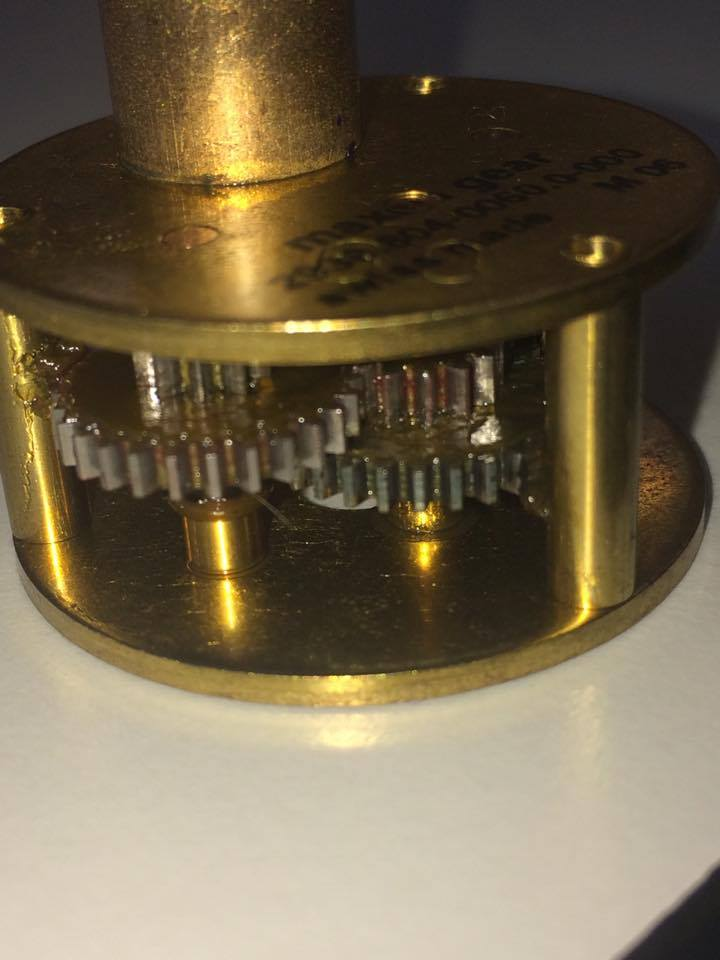
\includegraphics[trim = {0 9cm 0 6cm}, clip, width=\textwidth]{Gears_Before.jpg}
        \caption[Healthy Gears]{The gears of motor B before they were subject to any damage. Grease is visible on the cogs but no damage can be seen.}
    \end{subfigure}%
    ~ 
    \begin{subfigure}[t]{0.5\textwidth}
        \centering
         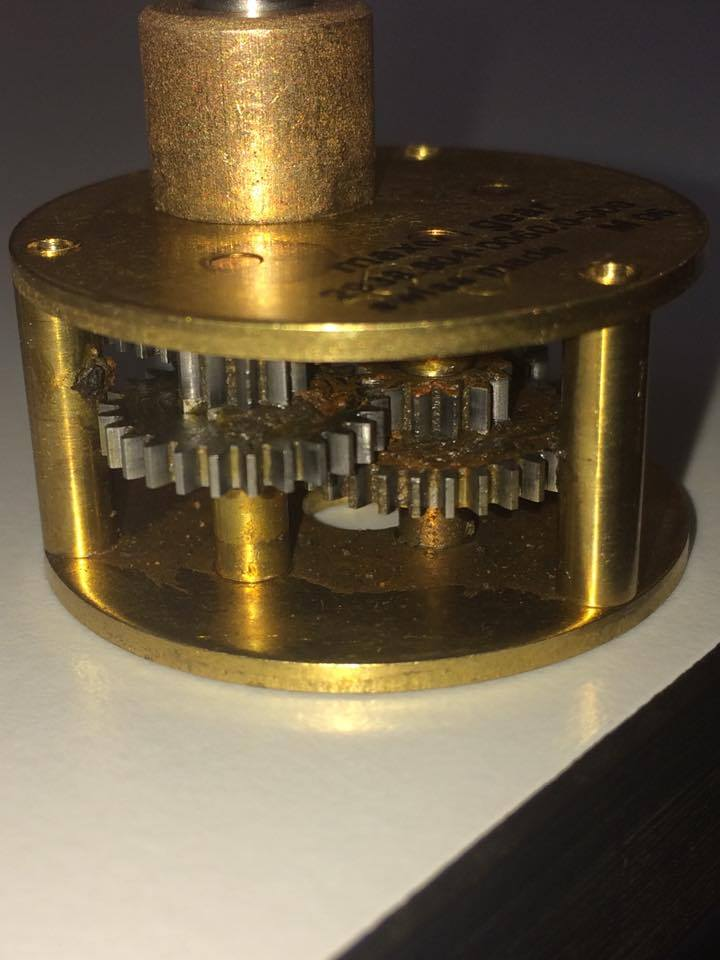
\includegraphics[trim = {0 9cm 0 6cm}, clip, width=\textwidth]{Gears_After.jpg}
    \caption[Damaged Gears]{The gears of motor B after they were degreased, placed in water and had mud added. Some rust can be seen on the top of each cog.}
    \end{subfigure}
    \caption[Motor Gears]{}
    \label{fig:gear_damage}
\end{figure*}

Gears are used to increase the torque of a motor so that it can take more load. The specific case relating rotation speeds of the axle and shaft for this motor is displayed in Equation.~\eqref{eq:gear_ratio}.

The gears of Motor B were damaged in ways so as to increase the friction inside the motor. This should raise the temperature, leading to overheating. One minute readings were taken before and after each separate attempt to deteriorate the motor. 

The first method used was to treat the gears with WD40. This was done several times to ensure gears were thoroughly cleaned.

They were then placed in water for 3 days so that they would rust. The effects of this could be seen on top of the cogs.

Finally dirt was added. This was an attempt to not only prevent easy movement, but also break some of the teeth. This can be seen in Figure.~\ref{fig:gear_damage}.

After each of these tests, it was audible that the gears were deteriorating. 


\subsubsection{Application of Anomaly Detection}

\begin{figure}[t]
    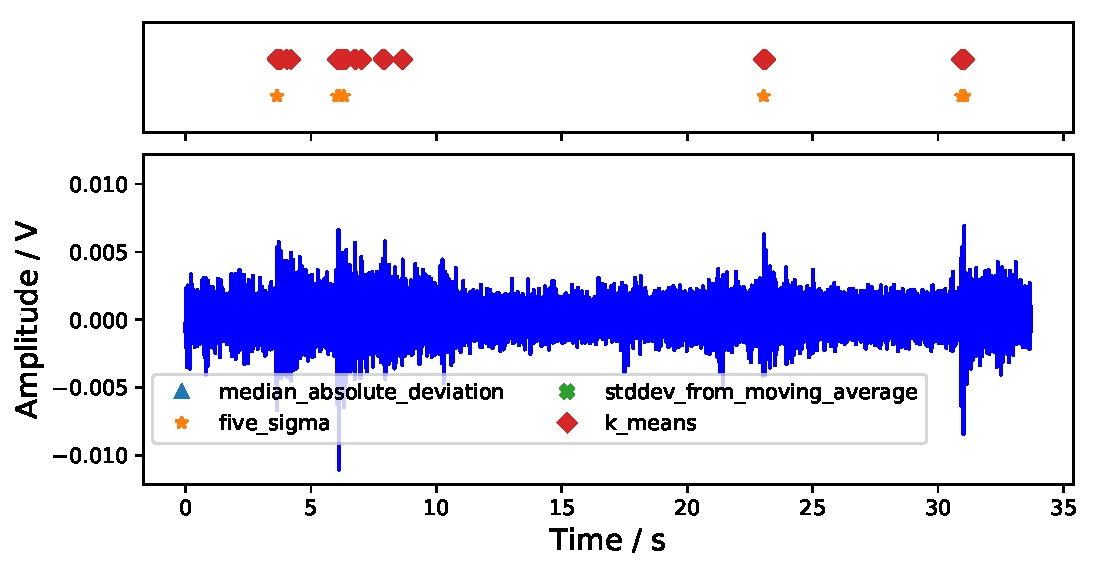
\includegraphics[width=1.0\textwidth]{fig/WD40_dry_dirt_12V_motornorm12V.pdf}
    \caption[Anomaly Tests 12 V Motor with Dirt]{The waveform for the 12 V motor in the x axis with WD40 applied to the gears and dirt added. Anomaly detection for K-means trained against baseline data at 12 V, which was assumed to be the motor's optimum working conditions.}
    \label{fig:12V_dirt}
\end{figure}

Following the treatment of WD40 the motor the data displayed no anomalies across the detection methods. Once the dirt was added inside the motor however anomalies began occurring, most likely due to the friction between the dirt and the moving parts of the motor which is as expected.

Figure.~\ref{fig:12V_dirt} shows that both the K-means and five sigma tests identified anomalies at similar times. The anomalies are visible in the waveform, and are probably caused by increased motor load as gear teeth have encountered a grain of dirt. 

At around the 5 second mark in Figure.~\ref{fig:12V_dirt}, it can be seen that the K-means test has successfully detected true anomalies for a longer time period that the five sigma test. This suggests that the K-means is more sensitive to true anomalies caused by interruptions in the gears of a motor.

%\begin{figure}[t]
%    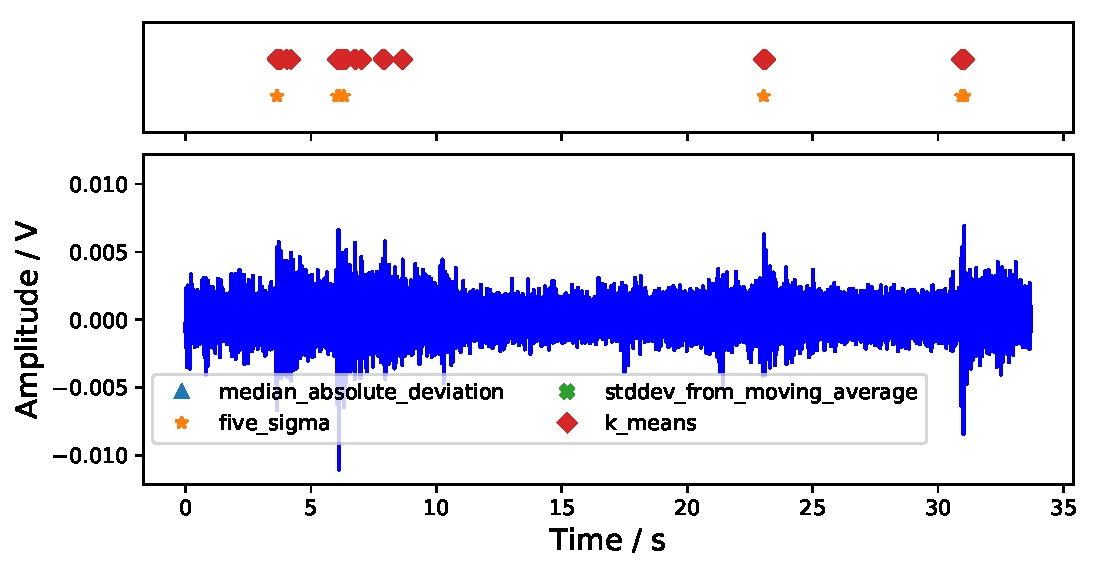
\includegraphics[width=1.0\textwidth]{fig/WD40_dry_dirt_12V_motornorm12V.pdf}
%    \caption[Anomaly Tests 30 V Motor with Paper Jam]{The waveform for the 12 V motor in the x axis run at 30 V, with gears de-greased and paper jammed in the rotor. Anomaly detection for K-means trained against baseline data at 12 V, which was assumed to be the motor's optimum working condition.}
%    \label{fig:12V_paper}
%\end{figure}

%\begin{figure}[t]
%    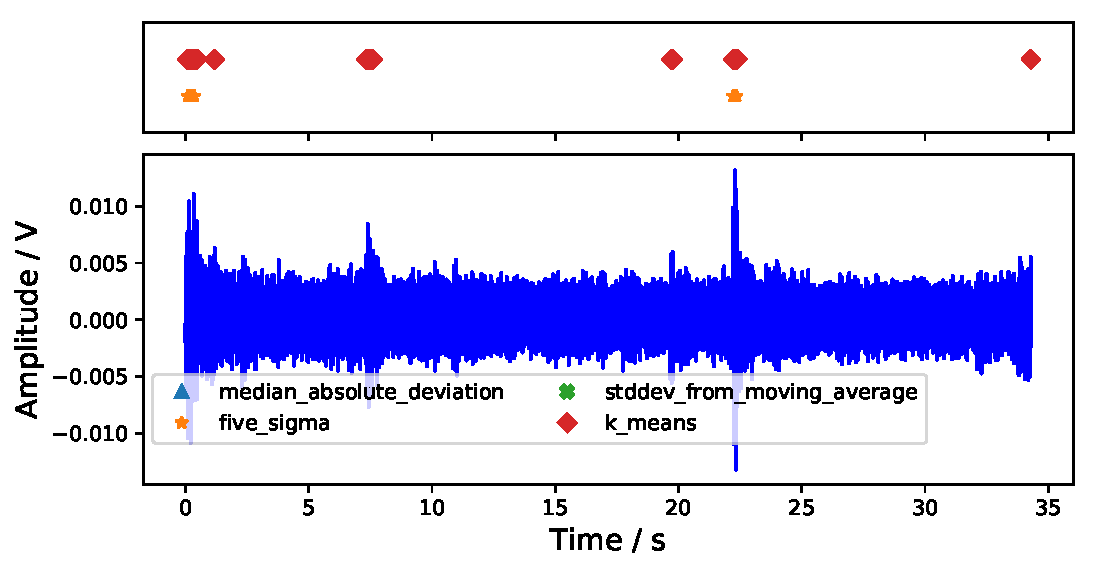
\includegraphics[width=1.0\textwidth]{fig/WD40_after_paper_12V_motornorm12V.pdf}
%    \caption[Anomaly Tests 12 V Motor after Paper Jam]{The waveform for the 12 V motor in the x axis run at 12 V, with gears degreased, after paper had been jammed in the rotor. Anomaly detection for K-means trained against baseline data at 12 V, which was assumed to be the motor's optimum working condition.}
%    \label{fig:12V_afterpaper}
%\end{figure}

%Not sure we should include the paper jamming here, could maybe go in specific anomalies?

\subsection{Soft Footing}

\subsubsection{Description of Failure Mode}
A motor running with soft footing can be the cause of multiple failures within a motor \cite{finley1999analytical}. When a motor with a misaligned shaft is coupled with an uneven motor housing, the uneven weight distribution as the rotor spins is exaggerated. The negative impacts of the uneven shaft are amplified, meaning even small misalignments can now be damaging. 

The cause of a soft footing can be either an imperfection in the mounting feet of the motor, or the foundations the motor is mounted upon. In either case the motor will have the ability to move in a diagonal plane, similar to a chair or table on uneven ground, causing the shaft to become misaligned. This can be avoided by properly aligning the mountings and the foundations, commonly performed in industry using laser precision tools. 

This failure mode was induced by suspending motor A above the work surface with a loosely gripped clamp stand. Any movement within the motor could cause a much larger movement in the stand, allowing the motor to oscillate while being suspended in the air. This oscillation will have an impact upon the shaft within the motor, exaggerating movements within the stator. The effects of this are similar to misalignment discussed above. Depending on the frequency of rotation of the motor, a resonance can occur, massively amplifying the oscillations causing an increased level of damage. If the feet do become loose, it is important to be aware of this before long term running of the motor is performed, as this would cause damage to internal components. It is more cost and energy effective to ensure proper footings prior to running.

\subsubsection{Application of Anomaly Detection}

\begin{figure}[t]
    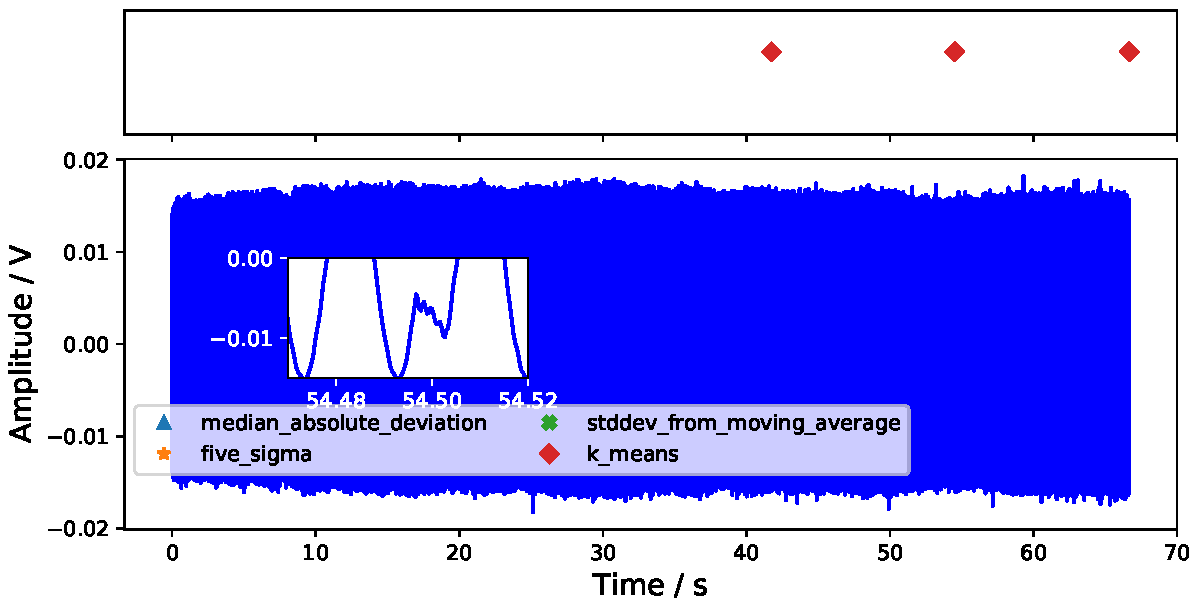
\includegraphics[width=1.0\textwidth]{fig/large_unlevel_large_12V.pdf}
    \caption[Anomaly Tests Large Motor Uneven Footing]{The waveform for the Motor A in the x axis with soft footing. Anomaly detection for K-means trained against 12 V baseline data, which was assumed to be the motor's optimum working conditions.}
    \label{fig:large_uneven_footing}
\end{figure}

Figure.~\ref{fig:large_uneven_footing} shows the waveform of Motor A in the x axis when it was run with soft footing. Only K-means detects anomalies. An inset axis shows a zoomed in view of one of the anomalies found by the K-means test. This shows the effectiveness of K-means and other reconstruction based methods in identifying changes in the shape of the waveform, instead of simply changes in amplitude. This shows the superiority of the K-means test above the simple statistical tests in detecting a variety of failure mode manifestations. 

However, a failing of K-means method is also shown in Figure.~\ref{fig:large_uneven_footing}, in that it detects a false positive for the last index of the waveform. This is due to the windowing of the synthetic segments used in K-means (see \S\ref{subsec:kmeans}), which has the effect of forcing each synthetic segment to begin and end with an amplitude of zero. If the waveform being reconstructed does not begin and end at an amplitude of zero, a large reconstruction error can result at the edges of the time series data, leading to a false positive.

%Talk about how only K-means fires, and finds a change int he SHAPE of the waveform, rather than just a change in amplitude. This is one big advantage of the reconstruction techniques compared to the simple statistical tests. Physically why would soft footing manifest itself like this?

\begin{figure*}[t!]
    \centering
    \begin{subfigure}[t]{0.5\textwidth}
        \centering
        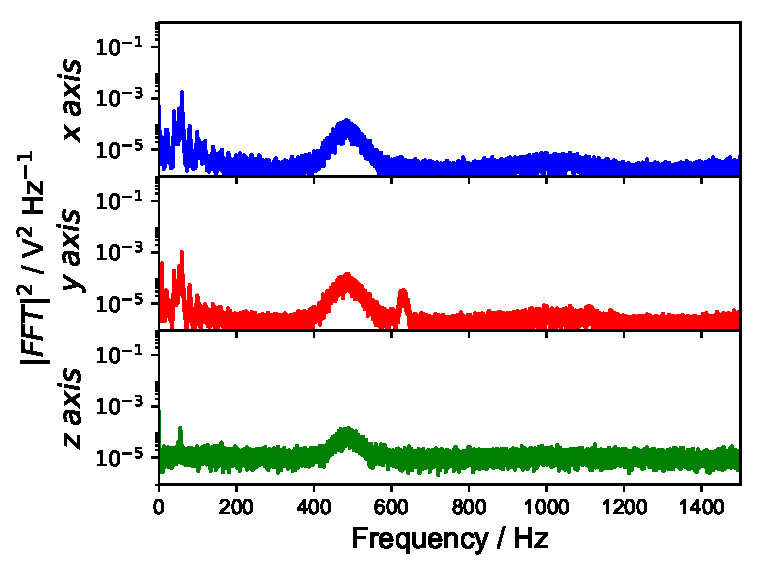
\includegraphics[height=2.5in]{freq_large_12V.pdf}
    \end{subfigure}%
    ~ 
    \begin{subfigure}[t]{0.5\textwidth}
        \centering
        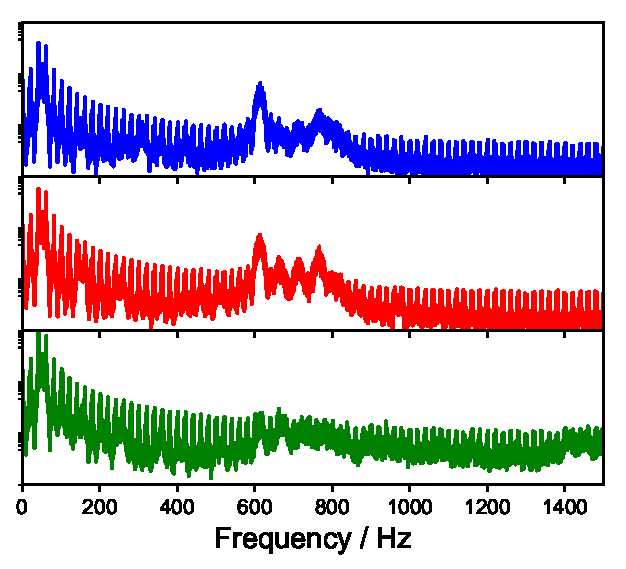
\includegraphics[height=2.5in]{freq_large_unlevel.pdf}
    \end{subfigure}
    \caption[Fourier Plot Soft Footing]{Fourier spectrum for Motor A. Left: baseline data in which motor was run at 12 V, which is assumed to be optimum running conditions. Right: Motor A with soft footing, simulated by suspending the motor within a loosely gripped clamp stand. }
    \label{soft_footing}
\end{figure*}

\vspace{20ex} %WATCH OUT THIS FORCES A MAGICAL PAGE BREAK
Following a loosening of the clamp stands on which the motor was running, a significant increase in power over all frequencies was detected. Very obvious harmonics are visible in Figure.~\ref{soft_footing} which are possibly associated with the fundamental frequency of the clamp stand. The peaks displayed on the $x$ and $y$ axes between 600 and 800 Hz are very pronounced, however, the peak on the $z$ axis lacks the same definition. This could be attributed to the motor having its movement more constricted along the $z$ axis. The increase in overall power across the frequencies makes physical sense due to the motor coming into and out of contact with the clamp at many different locations and times during the cycle.

%very obvious harmonics appearing, probably induced by motor being able to move more freely - might be harmonics associated with the fundamental frequency of the clamp stand. Peak between 600 and 800 Hz in x and y axis but not in z - why? Overall power over all frequencies much higher in general.

\subsection{Specific Failures}

\subsubsection{Description}

For testing purposes, to ensure that the various anomaly detection algorithms performed as expected, specific anomalies were induced. These included applying a force on the shaft, a routine of taps on the sensors or increasing and decreasing the voltage. The variations in frequencies induced by these actions are not found in a normal working motor, so the algorithm should detect these changes as anomalous. 

\subsubsection{Application of Anomaly Detection}

\begin{figure}[t]
    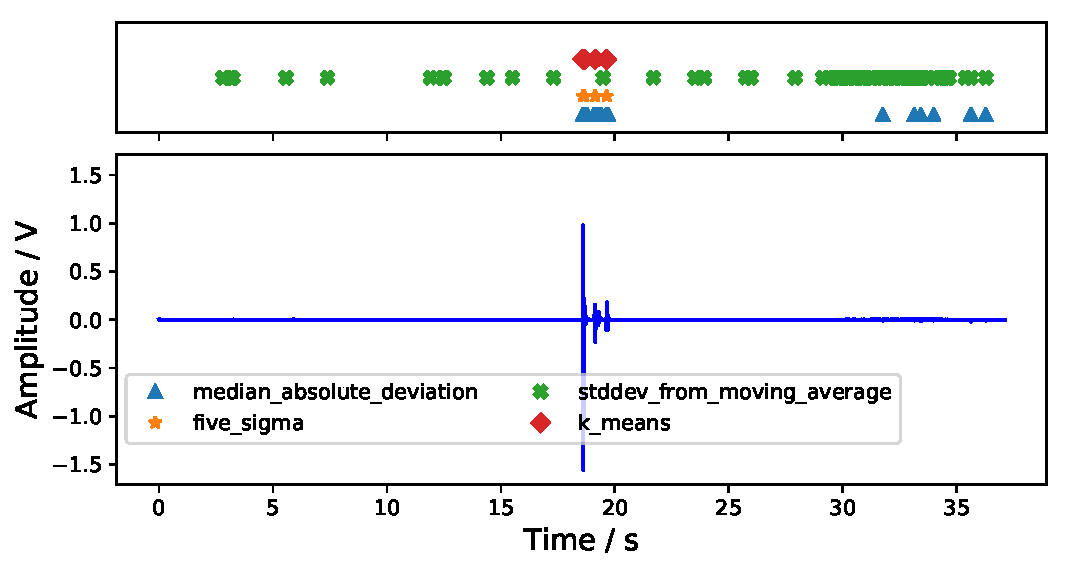
\includegraphics[width=1.0\textwidth]{fig/specific_anomaly_test1_motornorm12V.pdf}
    \caption[Specific Anomaly Test]{The waveform and detected anomalies in the x axis for the 12 V motor, with motors purposefully tapped at 30 seconds and voltage increased towards the end, in order to test the reliability of the anomaly detection methods being implemented.}
    \label{fig:spec_anom1}
\end{figure}

The detection of the obvious anomalous data by K-means, five sigma and median absolute deviation in Figure.~\ref{fig:spec_anom1} exhibits reliability in these particular methods. A point to note however is that K-means did not detect any anomalies as the voltage increases toward the end of the data set. This could be resolved by looking at the data within the Fourier domain to check if the anomaly detection methods including K-means detected the anomalies. 

Also, standard deviation from moving average did not manage to detect all of the obvious signs of anomalous data but did flag up the increasing voltage toward the end of the data. This shows a definitive advantage of using more than one anomaly detection method at once - that is to ensure that no single method misses an anomaly and the engine is damaged as a result.

%Talk about reliability of methods in finding anomalies. K-means doesn't find the increasing voltage at the end - perhaps showing important of fourier spectra for certain cases. 

\subsection{Commutator Damage}

\subsubsection{Description of Failure Mode}

As discussed earlier, a clean connection between the commutator and brushes is necessary for the healthy and efficient running of a DC motor. A disruption to this connection can be caused by either damage to the brushes, or the commutator. 

%\begin{figure*}[t!]
%    \centering
%    \begin{subfigure}[t]{0.5\textwidth}
%        \centering
%        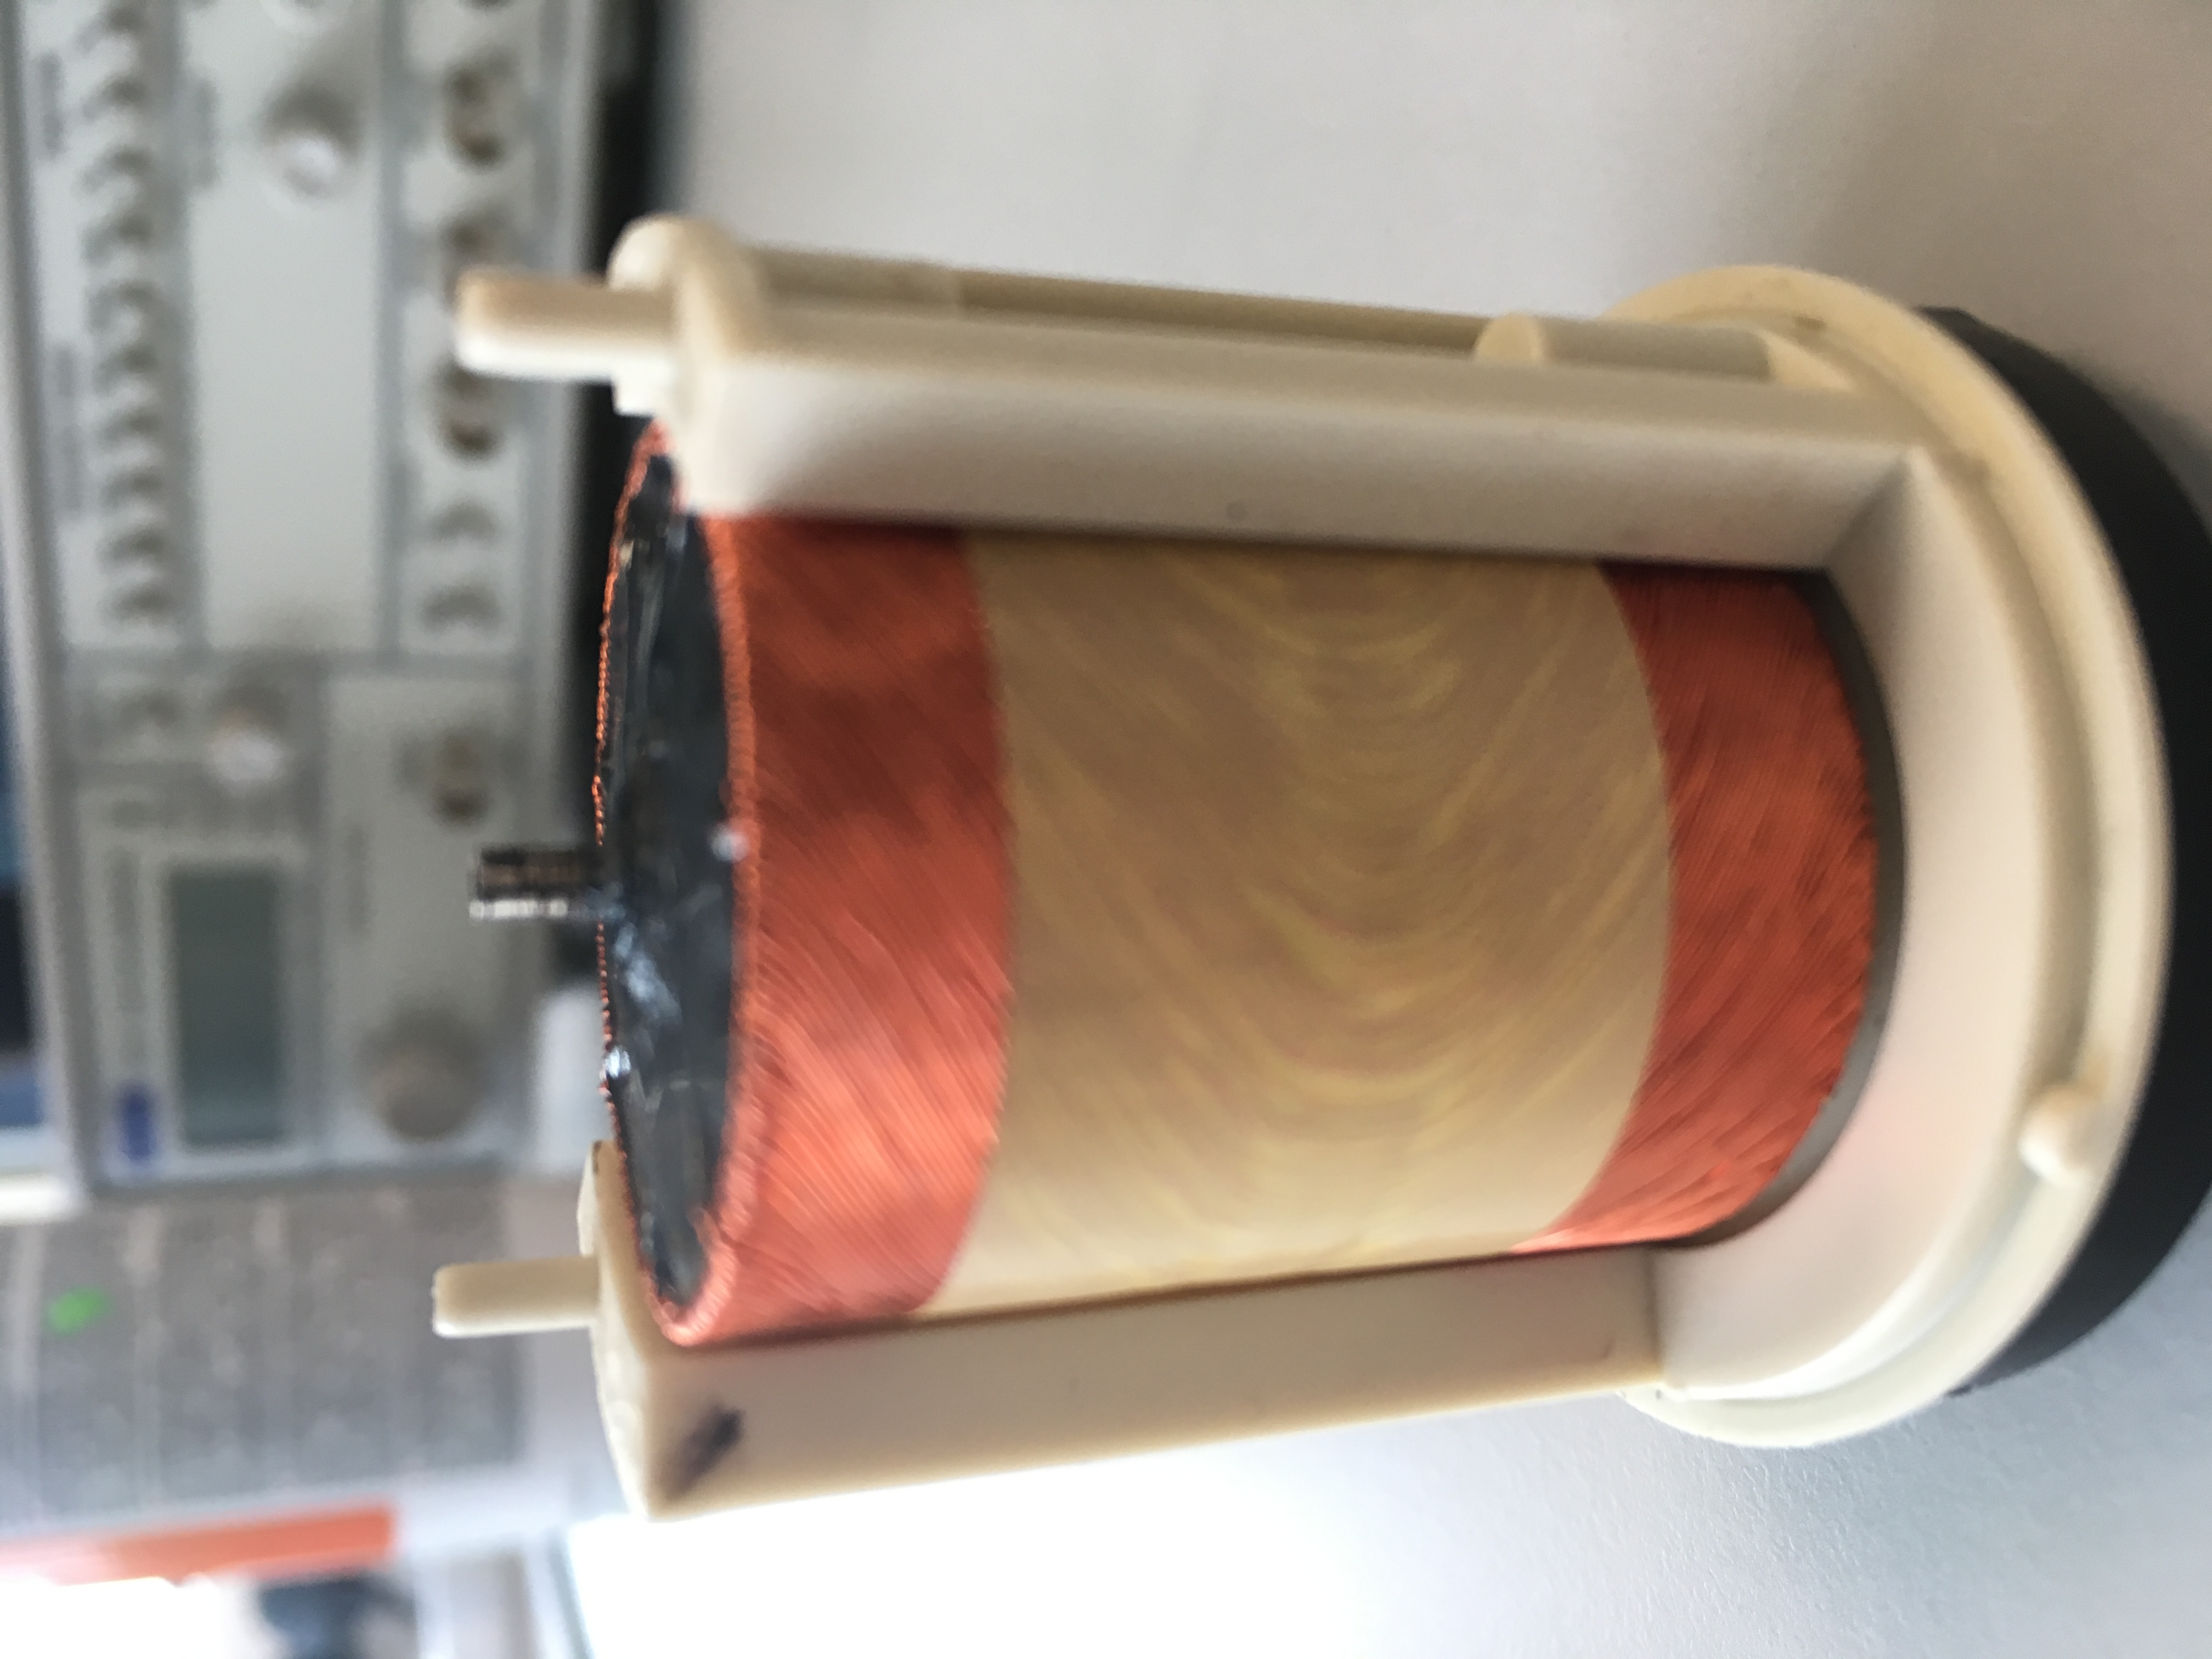
\includegraphics[trim = {0 9cm 0 6cm}, clip, width=\textwidth]{Commutator_Before.JPG}
%        \caption[Healthy Commutator]{The healthy commutator of motor B.}
%    \end{subfigure}%
%    ~ 
%    \begin{subfigure}[t]{0.5\textwidth}
%        \centering
%         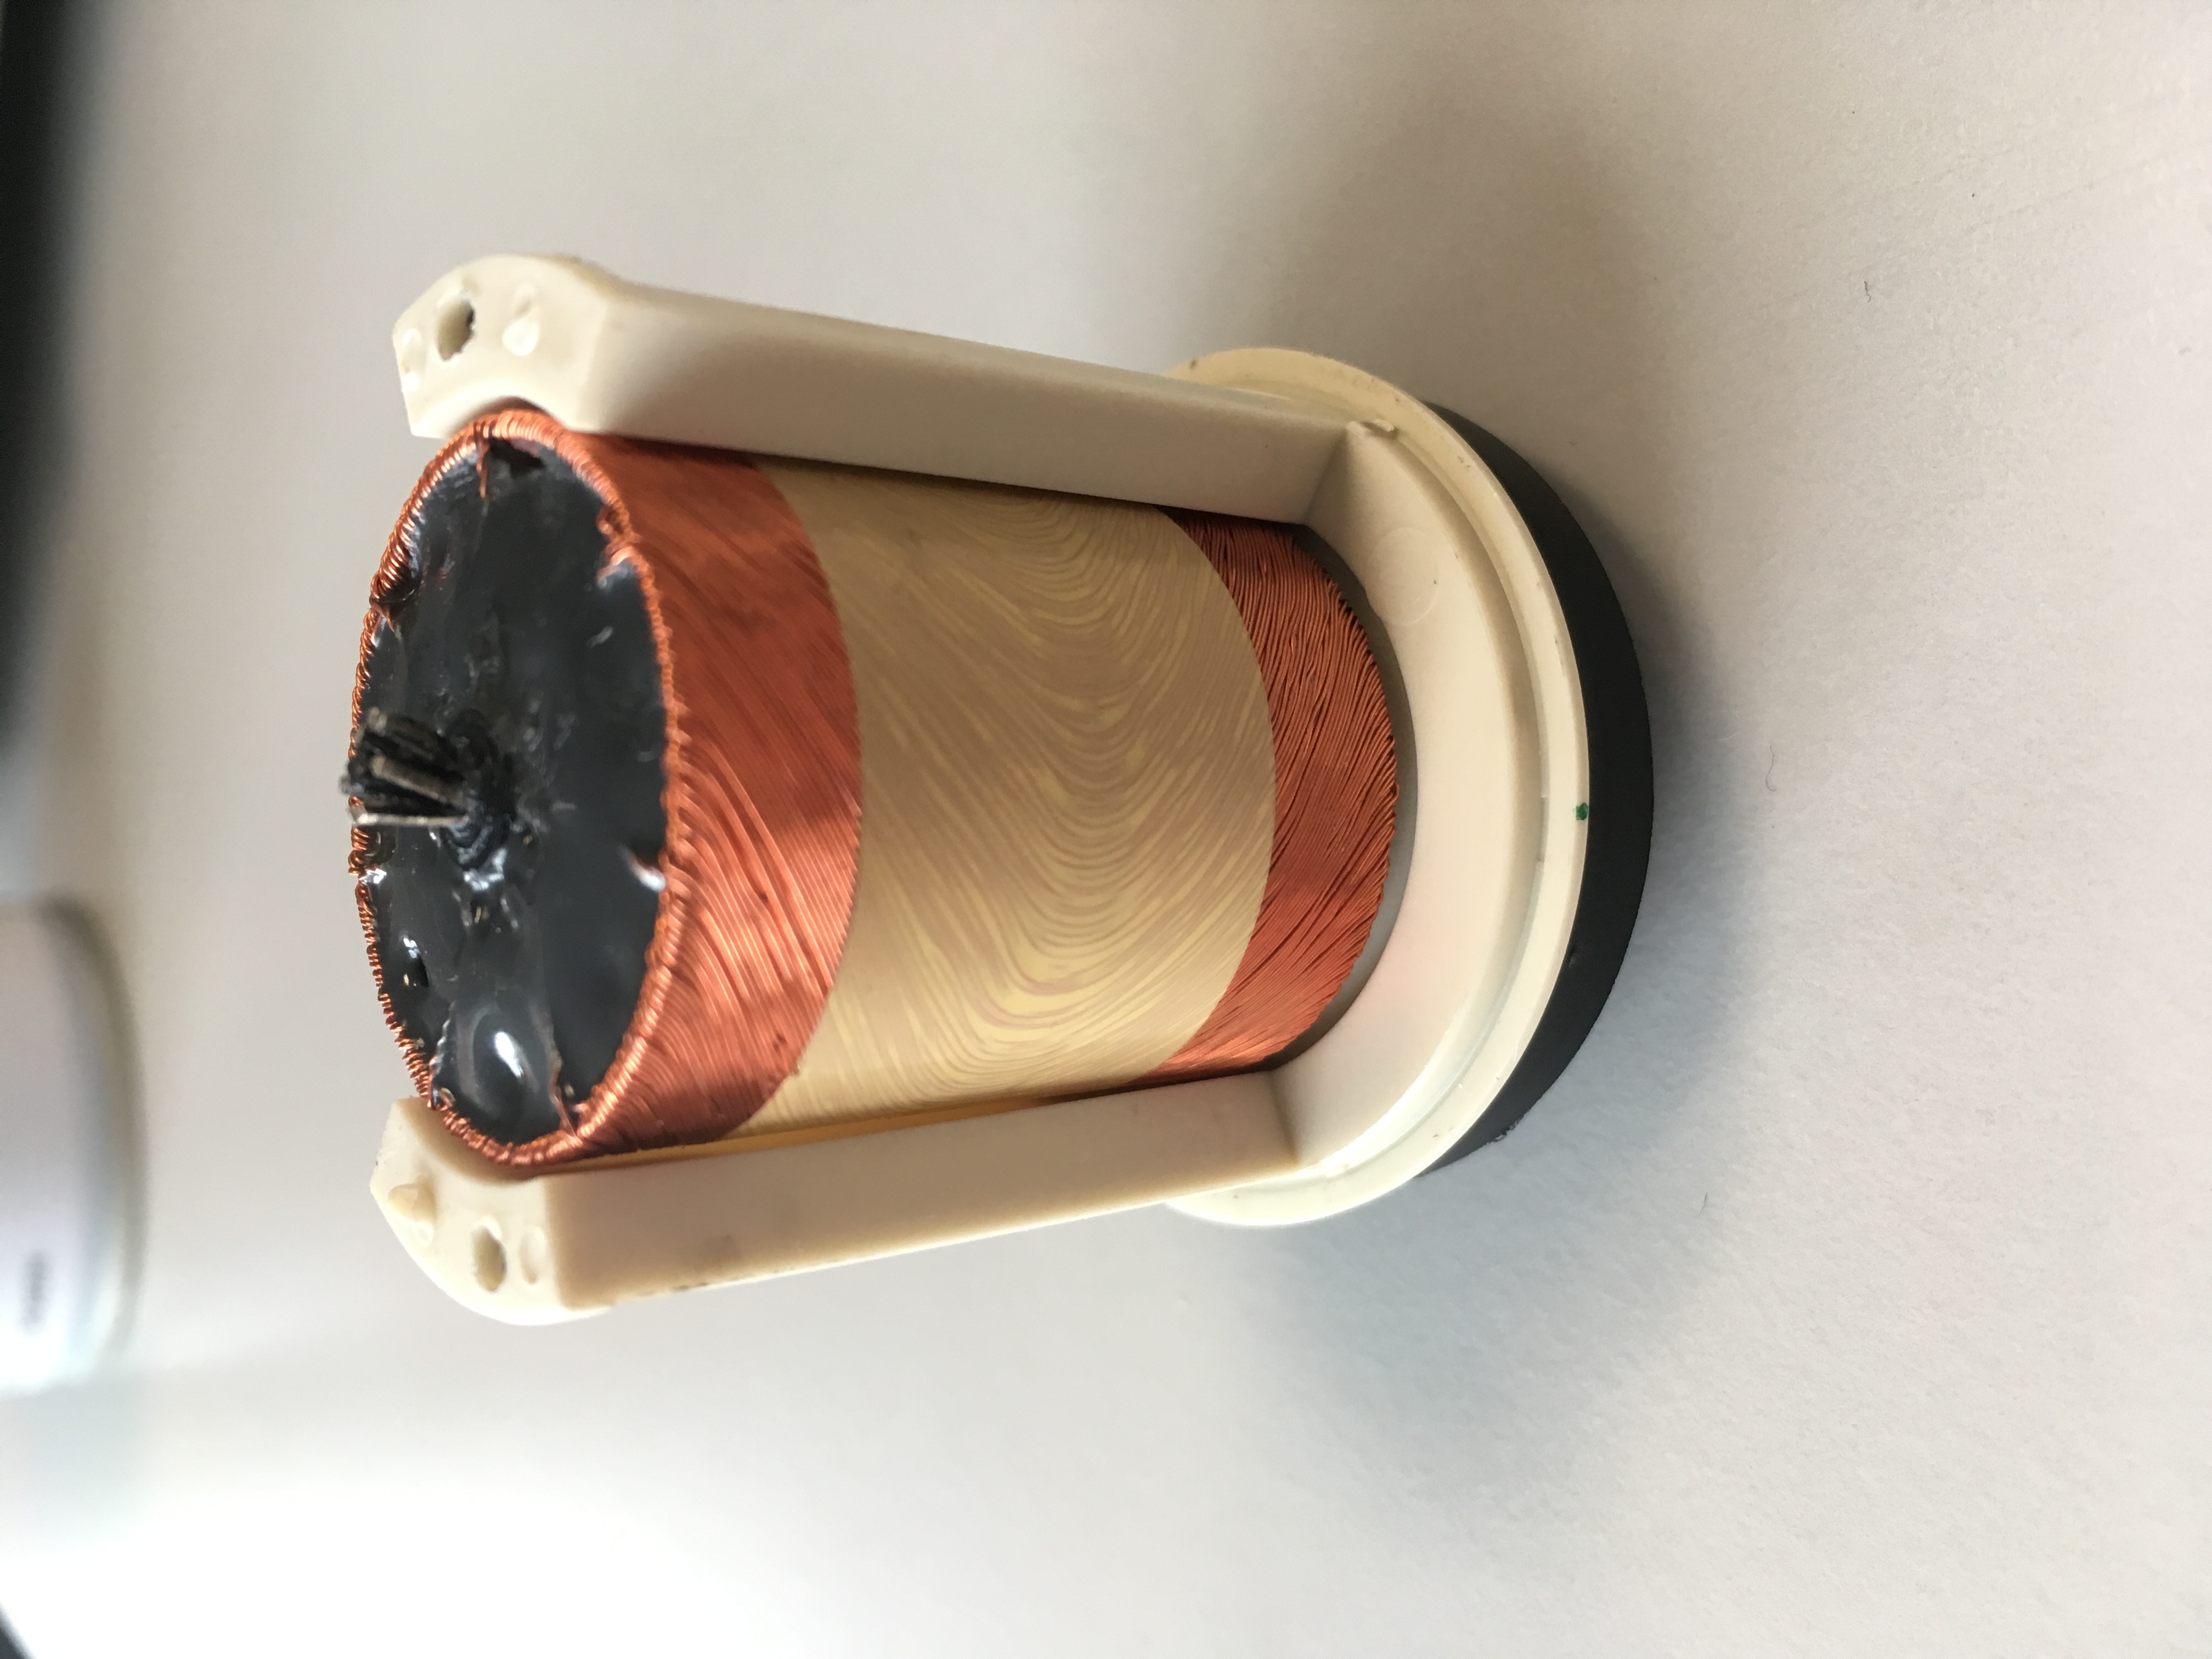
\includegraphics[trim = {0 9cm 0 6cm}, clip, width=\textwidth]{Commutator_After.JPG}
%    \caption[Damaged Commutator]{The commutator of motor B after impact force.}
%    \end{subfigure}
%    \caption[Motor Commutator]{}
%    \label{fig:commutator_damage}
%\end{figure*}

To simulate the effect of long term commutator damage, the commutators on motor B were impacted with a force. This deformed the commutator away from their ordinary shape, an extreme example of the types of damage that can manifest in a failing motor. The cause of this type of damage would usually be from some misalignment within the motor, requiring a mechanical movement. However sparking brushes from damaged carbon rods could also cause similar levels of harm to the connection. Replacing the commutator is a larger maintenance task, and this highlights the dangers of allowing a motor to run till it reaches this condition. If the other motor components are well maintained, this type of damage should not occur, it is therefore of utmost importance to ensure all motor components are operating at full health at all times.  

\subsubsection{Application of Anomaly Detection}

\begin{figure}[t]
    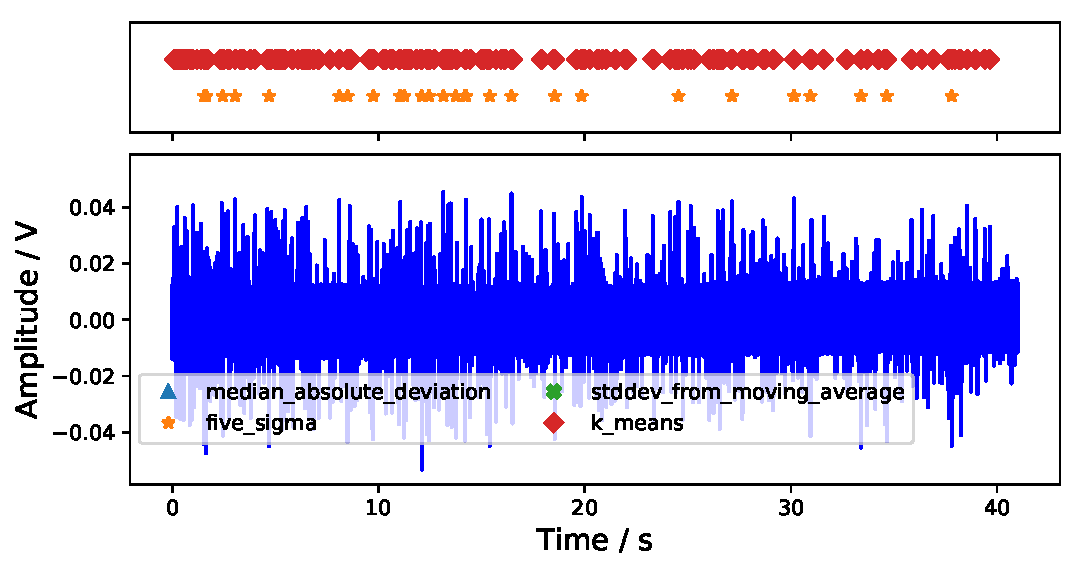
\includegraphics[width=1.0\textwidth]{fig/12V_hammer_motornorm12V.pdf}
    \caption[Anomaly Tests 12 V Commutator Damage]{The waveform for the 12 V motor after Commutator Damage}
    \label{fig:12V_Hammer}
\end{figure}

When the baseline data for the 12 V motor was passed through the anomaly detection methods no anomalous results were flagged up. This confirms that none of the anomaly indices flagged in Figure.~\ref{fig:12V_Hammer} are false positives and are all indeed anomalous data points. K-means method caught a very high number of anomalies in the set, however, five sigma flagged significantly less. This damage to the commutator clearly effects the physical operation of the motor, but shows no sign of self-repairing such as seen with damage to the brushes. Therefore it is imperative that the engine is switched off before any damage to the commutator arises.
%K-means catching everything. Not false positives as when applied to baseline data, no anomaly indices are returned. Link result with what would be expected to happen physically. 

